\documentclass[twoside]{article}

\usepackage{geometry}
\geometry{paperwidth=420mm,paperheight=297mm,left=0cm,right=0cm,top=.5cm,bottom=0cm}

\usepackage[PunctStyle=kaiming]{xeCJK}
\setCJKmainfont[Path=../fonts/,BoldFont=NotoSansCJKsc-Bold.otf]{NotoSansCJKsc-DemiLight.otf}
\setmainfont[Path=../fonts/,BoldFont=NotoSansCJKsc-Bold.otf]{NotoSansCJKsc-DemiLight.otf}
\newfontfamily{\Acumin}[Path=../fonts/]{AcuminExtraCondSemibold.otf}

\usepackage{xcolor}
\definecolor{lightblue}{HTML}{31c6f4}
\definecolor{darkblue}{HTML}{1f6899}

\usepackage{tikz}

\long\def\MakeCover#1#2#3#4{
    \def\halfthk{#1*0.025mm}
    \clearpage
    \begin{center}
        \begin{tikzpicture}
            \node[anchor=north west,inner sep=0] at (\halfthk-10mm,10mm) {
\includegraphics[width=175mm]{src/front.pdf}};
            \node[anchor=north east,inner sep=0] at (-\halfthk+10mm,10mm) {
\includegraphics[width=175mm]{src/back.pdf}};
            \node[anchor=north,inner sep=0] at (0mm,10mm) {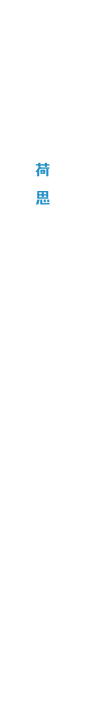
\includegraphics[width=30mm]{src/ridge.pdf}};
            
            \node[scale=3.67,white] at (\halfthk+77mm,-151mm) {\Acumin #2};
            \node[scale=3.67,white] at (\halfthk+77mm,-164mm) {\Acumin #3};
            \node[darkblue] at (-\halfthk-77.5mm,-174mm) {\parbox{75mm}{#4}};
            \node[anchor=north,darkblue,scale=1.6] at (0mm,-145mm) {\rotatebox{-90}{\Acumin #2}};
            \node[anchor=north,darkblue,scale=1] at (0mm,-155.7mm) {年};
            \draw[darkblue] (-2.5mm,-165mm) -- (2.5mm,-165mm);
            \node[anchor=north,darkblue,scale=1] at (0mm,-169.5mm) {第};
            \node[anchor=north,darkblue,scale=1.6] at (0mm,-173.2mm) {\rotatebox{-90}{\Acumin #3}};
            \node[anchor=north,darkblue,scale=1] at (0mm,-179.7mm) {期};

            \fill[lightblue] (-165mm-\halfthk,10mm)--(165mm+\halfthk,10mm)--(165mm+\halfthk,-10mm)--(-165mm-\halfthk,-10mm);
            \fill[darkblue] (-165mm-\halfthk,-245mm)--(165mm+\halfthk,-245mm)--(165mm+\halfthk,-225mm)--(-165mm-\halfthk,-225mm);

            \draw[thick]
                (-180mm-\halfthk,0mm)--(-170mm-\halfthk,0mm)
                (180mm+\halfthk,0mm)--(170mm+\halfthk,0mm)
                (-180mm-\halfthk,-235mm)--(-170mm-\halfthk,-235mm)
                (180mm+\halfthk,-235mm)--(170mm+\halfthk,-235mm)
                (-155mm-\halfthk,25mm)--(-155mm-\halfthk,15mm)
                (155mm+\halfthk,25mm)--(155mm+\halfthk,15mm)
                (-155mm-\halfthk,-260mm)--(-155mm-\halfthk,-250mm)
                (155mm+\halfthk,-260mm)--(155mm+\halfthk,-250mm)
                (-\halfthk,25mm)--(-\halfthk,15mm)
                (\halfthk,25mm)--(\halfthk,15mm)
                (-\halfthk,-260mm)--(-\halfthk,-250mm)
                (\halfthk,-260mm)--(\halfthk,-250mm); 
            % \draw (-\halfthk, 0mm) rectangle (\halfthk, -235mm);
            % \draw (-155mm-\halfthk, 0mm) rectangle (155mm+\halfthk, -235mm);
            % \draw (-165mm-\halfthk, 10mm) rectangle (165mm+\halfthk, -245mm);
        \end{tikzpicture}
    \end{center}
}
\def\fr{\mathfrak}
\def\det{\mathrm{det}}
\def\={\mathop{=}}
\def\rk{\mathrm{rk}}
\def\bar{\overline}
\def\check{\widecheck}
\def\hat{\widehat}
\def\bl{\textcolor{blue}}

\newcommand\dif{\mathop{}\!\mathrm{d}}  % 微分符号
\newcommand\real{{\mathbf{R}}}  % 实数集
\newcommand\abs[1]{\lvert#1\rvert}
\newcommand\VECTOR{\symbf}  % 向量
\newcommand\MATRIX{\symbf}  % 矩阵
\newcommand\vn{{\VECTOR{n}}}
\newcommand\vx{{\VECTOR{x}}}
\newcommand\mA{{\MATRIX{A}}}
\newcommand\mK{{\MATRIX{K}}}

\DeclareRobustCommand\cs[1]{\texttt{\char`\\#1}}
\providecommand\pkg[1]{{\sffamily#1}}

\usepackage{enumitem}
\setlist[enumerate, 1]{label=(\arabic*)}


\addbibresource{SM.bib}
\nocite{*}

\begin{document}

\title{A Study on Symmetric Manifolds}
\author{Luo Aoxue\footnote{罗傲雪}}

\begin{abstract}
Vertex algebras are algebraic structures that describe
the local data of a 2d chiral conformal field theory,
and its global data is described by conformal blocks.
Some conformal field theories arise as
chiral deformations of other theories,
and this construction corresponds
to the BRST reduction of a vertex algebra.
In this paper,
we propose a method of constructing families of
elements of the genus $1$ conformal block
for the BRST reduction of a vertex algebra.
This method is based on the technique of
regularized integrals of meromorphic forms on Riemann surfaces,
recently developed by Li and Zhou \cite{regularized}.
We show that
for an element of the conformal block,
its regularized integral against the BRST operator
gives an element of the conformal block
for the BRST reduction.
This provides a universal method of
constructing elements of BRST twisted conformal blocks geometrically.

\bigskip

\noindent
\textbf{Keywords:}
vertex algebra; conformal block; BRST reduction

\end{abstract}

\begin{center}
  \begin{tabular}{ll}
    \hline
    \textbf{Notation}              & \textbf{Definition} \\
    \hline
    $M$                            & smooth manifold,\\
    $G$                            & a Lie group,\\
    $\ssg$                         & the Lie algebra of $G$,\\
    $G_p$                          & the isotropy group(stabilizer) at $p$,\\
    $I(M)$                         & the isometry group of $M$,\\
    $I_0(M)$                       & the identity component of $I(M)$,\\
    $s_p$                          & the involution isometry at $p\in M$,\\
    $Gl(n,\mathbb{R})$             & $\{(n\times n) \text{ matrices } A \text{ over } \mathbb{R} \text{ with } \det A\neq 0\}$,\\
    $Sl(n,\mathbb{R})$             & $\{A \in Gl(n,\mathbb{R}) : \det A =1\}$,\\
    $SO(n)$                        & $\{A \in Sl(n,\mathbb{R}) : A^t=A^{-1}\}$,\\
    $\mathfrak {gl}(n,\mathbb{R})$ & $\{(n\times n) \text{ matrices } A \text{ over } \mathbb{R}\}$,\\
    $\mathfrak{sl}(n,\mathbb{R})$  & $\{X \in \mathfrak {gl}(n,\mathbb{R}) : \operatorname{tr} X=0\}$,\\
    $\mathfrak{so}(n)$             & $\{X \in \mathfrak {sl}(n,\mathbb{R}) : X^t=-X\}$. \\
    \hline
  \end{tabular}
\end{center}

\section{Introduction}

\hspace*{1em}
The thesis is to introduce the concept of (globally) symmetric manifolds. This is an important topic since many rigidity theorems are based on it. The advantage of this specific manifold is that the computation usually comes clear and easy, unlike some abstract manifold. Hence we turn to this topic.

Many people have already done quite a few work on it, including the authors of my reference books. They have classified different symmetric manifolds and have computed clearly. Since my learning is limited, I will only introduce some of the most important and basic knowledge and classification.

Next I would summarize the structure of the thesis. There are mainly four parts:
\begin{itemize}
    \item In chapter 2, I introduce some basic ideas of Lie groups and Lie algebras, which form a firm foundation of the advanced theories.
    \item In chapter 3, I formally introduce the concept of Riemannian symmetric manifold(space), and then discuss the properties and classification. There are several different statement of the classification of compact type, non-compact type and Euclidean type, and I will show the equivalence between them.
    \item In chapter 4, I introduce the concept of Hermitian symmetric manifold, which is not too much different from the Riemannian one. The de Rham decomposition theorem is still useful in the complex situation. And there is a borel embedding theorem worth to be known since it is useful.
    \item In chapter 5, I give some classical examples to show intuitively what a symmetric manifold is like.
\end{itemize}
The main reference of chapter 2 is \cite{Hel}, that of chapter 3 is \cite{Hel},\cite{Ziller},\cite{Besse}, and for chapter 4. it is \cite{Mok} and \cite{Ziller}. Examples in chapter 5 comes from several books including \cite{Peter},\cite{Ziller} and \cite{MR1451625}.











	 
	

\section{Prerequisites on Lie theories}

\subsection{Basic definitions}

Firstly, we want to learn the properties of the group of
isometries $I(M)$ of a manifold $M$. The goal is to reach the
identification between $M$ and $I(M)/I(M)_p\cong
I_0(M)/I_0(M)_p$, where the notations can be found in the
appendix or the following context.

We begin with basic definitions on Lie groups and Lie algebras.
If the reader is familiar with Lie theory, this section can be
skipped. Those who are not can simply read this section to get to
the advanced part.
\begin{definition}
	A Lie group is a group $G$ which is also a differential
	manifold such that the map $G\times G\to G,\
	(\sigma, \tau)\mapsto \sigma\tau^{-1}$ is smooth. A
	homomorphism of Lie groups is a homomorphism of groups which
	is smooth.
\end{definition}

\begin{definition}
	A Lie algebra $\mathfrak{g}$ over a field $k$ is a vector
	space over $k$  with a bilinear map
	$\mathfrak{g}\times\mathfrak{g}\to \mathfrak{g},\
	(X, Y)\mapsto [X, Y]$  such that
	
  \begin{enumerate}
    \item $[X,X]=0,\ \forall X\in \mathfrak{g} $,
    
    \item $[X, [Y, Z]]+[Y, [Z, X]]+[Z, [X, Y]]=0,\ \forall X, Y, Z\in \mathfrak{g}$.
  \end{enumerate}
	
	This bilinear map is also called the Lie bracket.
\end{definition}

\begin{theorem}
	Let $G$ be a Lie group. Then the tangent space of $G$ at $e$
	forms a Lie algebra over $\bbR$, usually called the Lie algebra
	of $G$, denote by Lie $G$, with the Lie bracket defined as
	$[X,Y]\\coloneq [\tilde X, \tilde Y]$, where $\tilde X, \tilde Y$ are
	the induced left-invariant vector fields by $X, Y$, and the
	Lie bracket is the standard one for vector fields.
\end{theorem}

\begin{definition}
	Let $\ssg$ be a Lie algebra over field $k$. A Lie subalgebra
	of it $\ssl$ is a vector space  with $[\ssl, \ssl]\in \ssl$,
	where $[\ssm, \ssn]$ is the vector space generated by all the
	elements $[X, Y]$, $X\in \ssm, Y\in \ssn$.
\end{definition}

\begin{definition}
	A homomorphism of Lie algebras from $\ssg$ to $\ssm$ is a
	linear map $f\:\ssg\to \ssm$ such that $[fX, fY]=f[X, Y]$.
\end{definition}
\begin{definition}
	Let $G$ be a Lie group and $ \nabla$ be an affine connection
	on $G$. $\nabla$ is called left invariant on $G$ is for any
	vector fields $X,Y$ on $G$ and $g\in G$, there is an equality
	$\nabla_{dL_gX}(dL_gY)=dL_g(\nabla_XY)$.
\end{definition}
\begin{lemma}
	Every left-invariant vector field on a Lie group is complete.
\end{lemma}
\bproof
See \cite{Lee} Cor 9.17.
\eproof
\subsection{The exponential map}

Next we define the exponential map on a Lie group.

\begin{lemma}\label{8}
	There is a one-to-one correspondence between the set of
	left-invariant affine connections $\nabla$ on $G$ and the set
	of bilinear functions $\alpha$ on $\ssg\times\ssg$ with
	values in $\ssg$ given by
	\[ \alpha(X, Y)=(\nabla_{\tilde X}\tilde Y)_e \]
	where $\tilde X, \tilde Y$ are the induced left-invariant vector fields by
	$X, Y$. Moreover, for a given bilinear function $\alpha$(and
	left invariant affine connection $\nabla$) and $X\in \ssg$,
	the following are equivalent:
	
  \begin{enumerate}
	  \item $\alpha(X, X)=0$;
	
	  \item The geodesic $t\to \gamma_X(t)$ is a smooth homomorphism
	of $\bbR$ into $G$.($\gamma_X(t)$ indicates the geodesic
	$\gamma(t)$ with $\gamma(0)=e, \gamma'(0)=X$.)
  \end{enumerate}
	\bproof
	Given a bilinear mapping $\alpha$, we defined the affine
	connection by
	\[
	\nabla_{\tilde{E_i}}\tilde{E_j}=\tilde{\alpha(E_i,E_j)},
	1\le i,j\le n
	\]
	where $\{E_i\}_{i=1}^n$ is an arbitrary basis of the tangent
	space of $G$ at $e$. Then the correspondence follows.
	
	Next it comes to the equivalence. If $\alpha(X,X)=0$, then
	$(\nabla_{\tilde X}\tilde{X})_e=0$, and $\nabla_{\tilde
	X}\tilde{X}=0$ by the left invariance of $\nabla$.
	
	Let $\gamma\:\bbR\to G$ be the integral curve of $\tilde{X}$
	starting at $e$. Then $\gamma $ is a geodesic. For any $s\in
	R$, the curves $t\to \gamma(s+t)$ and $t\to
	\gamma(s)\gamma(t)$ are both geodesics since $\nabla$ is left
	invariant. These two curves have tangent vectors $\gamma'(s)$
	and $dL_{\gamma(s)}X$ at $t=0$. So by uniqueness,
	$\gamma(s+t)=\gamma(s)\gamma(t)$. On the other hand, suppose
	$\gamma_X\:\bbR\to G$ is a smooth homomorphism, then by
	$\gamma_X(s+t)=\gamma_X(s)\gamma_X(t)$, we have
	$\gamma_X'(s)=\tilde X_{\gamma_X(s)}$ for all $s\in \bbR$. So
	$\nabla_{\tilde X}\tilde{X}=\nabla_{\gamma_X'}\gamma_X'=0$ on
	$\gamma_X$ and $\alpha(X,X)=(\nabla_{\tilde
	X}\tilde{X})_e=0$.
	\eproof
\end{lemma}
\begin{corollary}\label{9}
	Let $G$ be a Lie group and $\ssg$ be its Lie algebra. For any
	$X\in \ssg$, there exists a unique smooth homomorphism
	$\theta\:\bbR\to G$ such that $\theta'(0)=X$.
\end{corollary}
\bproof
Let $\alpha$ be a bilinear form on $ssg$ such that
$\alpha(X,X)=0$ and $\nabla$ is the left invariant affine
connection correspondingly. Let $\gamma_X\:\bbR\to G$ be the
geodesic as in lemma $\ref{8}$. Then, for any smooth homomorphism
$\theta$ with $\theta'(0)=X$, similarly as the proof of lemma
$\ref{8}$, we have $\theta(s+t)=\theta(s)\theta(t)$. Then
$\theta'(t)=dL_{\theta(t)}\theta'(0)=dL_{\theta(t)}X$ and
$\nabla_{\theta'}\theta'=\nabla_{\tilde X}\tilde
X=dL_{\theta(t)}(\nabla_{\tilde X}\tilde X)_e=0$. Hence $\theta$
is a geodesic with $\theta'(0)=X$, so by uniqueness of geodesic,
$\theta=\gamma_X$.
\eproof
\begin{definition}
	Let $G$ be a Lie group and $\ssg$ be its Lie algebra. The
	exponential map $\exp\:\ssg\to G$ is defined to be $\exp X =
	\theta_X(1)$, where $\theta_X$ is the unique smooth
	homomorphism from $\bbR$ to $G$ such that $\theta_X'(0) = X$.
\end{definition}

By now we have known the definition of an exponential map on a
Lie group. The following lemma is a basic and useful property
related.

\begin{lemma}
	Let $H$ and $K$ be Lie groups with Lie algebras $\ssh$ and
	$\ssk$ respectively. Let $\phi$ be a smooth homomorphism from
	$H$ to $K$. Then $d\phi_e$ is a homomorphism from $\ssh$ to
	$\ssk$ and
	\[\phi(\exp X)=\exp d\phi_e(X), \forall X\in \ssh.\]
\end{lemma}
\bproof
Let $X \in \ssh$. The mapping $t \to \phi(\exp tX)$ is a smooth
homomorphism of $\bbR$ into $K$. If we put $X' = d\phi_e(X)$,
corollary $\ref{9}$ implies that $\phi(\exp tX) = \exp tX'$ for
all $t \in R$. Since $\phi $ is a homomorphism, we have
$\phi(\sigma\tau) = \phi(\sigma)\phi(\tau)$. Hence $\phi\circ
L_{\sigma}=L_{\phi(\sigma)}\circ\phi$ for $\sigma \in H$. It
follows that $d\phi_{\sigma}\circ
dL_{\sigma}(X)=dL_{\phi(\sigma)}(X')$. Then
$d\phi_{\sigma}(\tilde X_{\sigma})=\tilde X_{\phi(\sigma)}'$.
This means that the left invariant vector fields $\tilde{X}$ and
$\tilde X'$ are $\phi $ related. So $[\tilde X', \tilde
Y'](\phi(\sigma))=d\phi_{\sigma}([\tilde X, \tilde Y](\sigma))$
and $[X', Y']=[d\phi_eX, d\phi_eY]=d\phi_e[X, Y]$. Hence
$d\phi_e$ is a homomorphism between Lie algebras and the lemma is
shown.
\eproof
\subsection{Lie subgroups and subalgebras}

Then it comes to the part of Lie subgroups and Lie subalgebras.
The following are also basic knowledges but are essential for
building the whole theory.

\begin{definition}
	Let $G$ be a Lie group. $H$ is called a Lie subgroup if it is
	an immersed submanifold $H$ such that
	
  \begin{enumerate}
    \item $H$ is a subgroup of group $G$;
    
    \item $H$ is a topological subgroup.
  \end{enumerate}
\end{definition}

 We see that a Lie subgroup is itself a Lie group by definition.

\begin{theorem}
	Let $G$ be a  Lie group and $H$ be its arbitrary Lie
	subgroup. Suppose $\ssg$ and $\ssh$ are their Lie algebras
	respectively,
	then
	 $\mathfrak{h}$ is a subalgebra of $\mathfrak{g} .$ Moreover,
	 each Lie subalgebra of $\ssg$ is the Lie algebra of a unique
	 connected Lie subgroup of $G$.
\end{theorem}
\bproof See \cite{Hel} Theorem 2.1 Chapter II.
\eproof
\begin{theorem}
	Let $G$ be a Lie group,  Lie $G=\ssg$ , and $H$ be a
	subgroup. Suppose $H$ is a closed subset of $G$, then there
	exists a unique smooth
	structure of ${H}$ such that it is a topological subgroup of
	$G$.
\end{theorem}
\bproof
See \cite{Hel} Theorem $2.3$ Chapter II.
\eproof

\begin{definition}
	A topological group $G$ is a group endowed with a topology
	such that the mapping $(\sigma, \tau) \mapsto \sigma
	\tau^{-1}$ from $G \times G$ to $G$ is continuous. A
	topological subgroup $H$ of $G$ is a subgroup endowed with
	the subspace topology such that it is a topological group.
\end{definition}

Next we define Lie transformation groups.
\begin{definition}
Let $M$ be a Hausdorff space. A topological transformation group
$G$ is a topological group such that each $g \in G$ is associated
with a homeomorphism $p \rightarrow g \cdot p$ of $M$ onto itself
such that

\begin{enumerate}
  \item $\left(g_{1} g_{2}\right) \cdot p=g_{1} \cdot \left( g_{2}
\cdot p \right)$,

  \item the mapping $(g, p) \mapsto g \cdot p$ is a continuous
mapping of the product space $G \times M$ to $M$.
\end{enumerate}

If for any $p, q \in M$, there exists $g \in G$ such that $g
\cdot p=q$, then we say $G$ is transitive on $M$.	
\end{definition}
\subsection{quotient manifolds}

The next two theorems shows how we see a coset space $G / H$ as a
topological manifold.

\begin{theorem}
	Let $G$ be a topological group and $H$ a closed topological
	subgroup of $G$. Then the set $G / H$ can be endowed
	with the quotient topology to be a Hausdorff space, and also
	the natural projection $\pi\: G \rightarrow G / H$ is open
	and continuous. $G$ acts naturally on $G / H$ by $\mathrm{g}
	\cdot {\sigma H}={g} \sigma {H}$ and $\mathrm{G}$ is a
	topological transformation group on ${G} /{H}$.
\end{theorem}
\bproof
See \cite{Hel} p120 for example. 
\eproof

\begin{theorem}
	Let $G$ be a locally compact group which is a topological
	manifold. Suppose $G$ is a transitive topological
	transformation group of a locally compact Hausdorff space
	$M$. Let $p$ be any point in $M$ and $H$ the subgroup of $G$
	which leaves $p$ fixed. Then ${H}$ is closed and the mapping
	\[
	g H \rightarrow g \cdot p
	\]
	is a homeomorphism of $G / H$ onto $M$.
\end{theorem}
\bproof
See \cite{Hel} Theorem $3.2$ Chapter II.
\eproof
\begin{definition}
	Let $G$ be a Lie group and $M$ a differential manifold.
	Suppose $G$ is a topological transformation group of $M .\bbG$ is
	called a Lie transformation of $M$ if the mapping $(g, p)
	\mapsto g \cdot p$ is a differentiable mapping from $G \times
	M$ to $M$.
\end{definition}

From the definition we see that a Lie transformation group adds a
differentiable condition from a topological one. The next theorem
shows the equivalence between $G / H$ and a smooth manifold under
this new condition.

\begin{theorem}
Let $G$ be a Lie group and $H$ a closed subgroup.  The space $G / H$
of left cosets $g H$ with the natural topology. Then $G / H$ ha
s a unique smooth structure with the property that $G$ is a Lie
transformation group of $G / H$.	
\end{theorem}
\bproof
See \cite{Hel} Theorem 4.\ 2, Chapter II.
\eproof

\begin{proposition}
	Let $G$ be a transitive Lie transformation group of a
	$C^{\infty}$ manifold $M$. Let $p_{0}$ be a point in $M$ and
	let $G_{p_{0}}$ denote the isotropy group of $G$ that leaves
	$p_{0}$ fixed. Then $G_{p_0}$ is closed. Let $\alpha$ be the
	mapping
	\[
	\alpha\:g G_{p_{0}} \rightarrow g \cdot p_{0} \text { of \
	}\  G / G_{p_{0}} \text { onto } M.
	\]
	If $\alpha$ is a homeomorphism, then it is a diffeomorphism (
	$G / G_{p_{0}}$ having the analytic structure defined above).
\end{proposition}
\bproof
See \cite{Hel} Proposition 4.\ 3 Chapter II.
\eproof
\subsection{The group of isometries}

Finally, we start to learn the properties of $I(M)$ as a Lie
group. To begin with, we need to know its topology. 

\begin{definition}
	Let $M$ be a Riemannian manifold and $I(M)$ be the group of
	all isometries of
	M. The compact open topology on $I(M)$ is defined as the
	smallest topology on $I(M)$ for which all the sets
	\[
	W(C, U)\\coloneq \{ g \in I(M) \mid g (C) \subset U \}
	\]
	where $C \subset M$ is a compact subset and $U \subset M$ is
	an open subset.
\end{definition}
\begin{lemma}
	The space $I(M) $ is second countable.
\end{lemma}
\bproof
See \cite{Hel} Lemma 2.\ 1 Chapter IV.
\eproof
\begin{lemma}
	Assume that a sequence $\left\{ f_{n}
	\right\}_{n=1}^{\infty}$ in $I(M)$ converges pointwisely on a
	set $A \subset M$. Then $\left\{ f_{n}
	\right\}_{n=1}^{\infty}$ also converges pointwisely on
	$\bar{A}$.
\end{lemma}
\bproof
See \cite{Hel} Lemma $2.3$ Chapter IV.
\eproof
\begin{lemma}
	Let $M$ be a Riemannian manifold and $\left\{ f_{n} \right\}$
	be a sequence in $I(M) .$ Suppose there exists a point $p \in
	M$ such that $\left\{ f_{n} (p) \right\}$ converges in $M$.
	Then there exists a subsequence $\left\{f_{n_{k}}\right\}$ of
	$\left\{f_{n}\right\}$ converging pointwisely.
\end{lemma}
\bproof
See \cite{Hel} Theorem $2.2$ Chapter IV.
\eproof
\begin{theorem}
	Let $\left\{ f_{n} \right\}$ be a sequence in $I(M)$, then
	$\left\{ f_{n} \right\}$ converges pointwisely on $M$ if and
	only if $\left\{ f_{n} \right\}$ converges to some $f \in I(M)$
	in the compact open topology.
\end{theorem}
\bproof
See \cite{Hel} Lemma 2.\ 4 Chapter IV.
\eproof
\begin{theorem}
	Let $M$ be a Riemannian manifold. Then $I(M)$ is a locally
	compact topological
	transformation group of $M$ with respect to the compact open
	topology on $I(M)$. Moreover, the stabilizer  $I(M)_p$  is
	compact for all $p \in M$.
\end{theorem}
\bproof
See \cite{Hel} Theorem 2.\ 5 Chapter IV.
\eproof


\section{Riemannian symmetric manifolds}

\subsection{Basic definitions}

Now we introduce the theory of symmetric manifolds (or called
symmetric spaces). Firstly we give some basic geometric
properties, learning more about $I(M)$ in passing.

\begin{definition}
Let $M$ be a Riemannian manifold. $M$ is a  Riemannian (globally)
symmetric
if each $p \in M$ is an isolated fixed point of an involutive
isometry $s_{p}$ of $M$.	
\end{definition}
\begin{definition}
	A mapping is called involutive if its square, but not the
	mapping itself, is
	the identity.
\end{definition}
For an isometry, it has the following properties:
\begin{lemma}\label{31}
	Let $\left( M, g_{M} \right)$ and $\left( N, g_{N} \right)$
	be two Riemannian manifolds and $F\: M \rightarrow N$ be a
	local Riemannian isometry. Then
	
  \begin{enumerate}
    \item $F$ maps geodesics to geodesics.
    
    \item For any $p \in M$ and $v \in T_{p} M$, if $\exp _{p} v$
    is defined, then $\exp _{F(p)}\left( D F_{p}(v) \right)$ is
    defined and $F \circ \exp _{p}(v) = \exp _{F(p)} \circ D
    F_{p}(v) .$ \qedhere
  \end{enumerate}
\end{lemma}
\bproof \hfill
\begin{enumerate}
  \item is an obvious conclusion in Riemannian geometry.

  \item If $\exp _{p}(v)$ is defined, then $t \mapsto \exp _{p}(t v)$
  is a geodesic. Thus $t \mapsto$ $F\left( \exp _{p}(t v) \right)$
  is also a geodesic. Since
  \[
  \begin{aligned}
    \left.\frac{d}{d t} F\left( \exp _{p}
    \right)\right|_{t=0} &=D F\left( \left .\frac{d}{d t} \exp
    _{p}(t v) \right|_{t=0} \right) =D F(v)
  \end{aligned}
  \]
  we have that $F\left( \exp _{p}(t v) \right)=\exp _{F(p)}(t D
  F(v))$. Setting $t=1$ then the claim is proved.
\end{enumerate}
\eproof
\begin{corollary}\label{11.2}
Let $F, G\:\left( M, g_{M} \right) \rightarrow \left( N, g_{N}
\right)$ be two local Riemannian isometries. If $M$ is connected
and there exists $p \in M$ such that $F(p) = G(p), D F_{p} = D
G_{p}$, then
$F=G$ on $M$.	
\end{corollary}
\bproof
Let
\[
A=\left\{ x \in M \mid F(x) = G(x), D F_{x} = D G_{x} \right\}
\]
We know that $p \in A$ and that $A$ is closed. Property (2) of
Lemma $\ref{31}$ tells
that
\[
\begin{aligned}
	F \circ \exp _{x}(v) & = \exp _{F(x)} \circ D F_{x}(v) =\exp
	_{G(x)} \circ D G_{x}(v) = G \circ \exp _{x}(v)
\end{aligned}
\]
if $x \in A$. Since $\exp _{x}$ maps onto a neighborhood of $x$
it follows that some
neighborhood of $x$ also lies in $A$. This shows that $A$ is open
and hence 
$A=M$ by connectedness.
\eproof

\begin{theorem}
	Let $M$ be a Riemannian globally symmetric manifold. Then $M$
	is geodesically complete and for any $p \in M$ and any
	involutive isometry $s_{p} \in I(M)$ with $p$ as an isolated
	fixed point, it holds that $s_{p}\left( \exp _{p} v
	\right)=\exp _{p}(-v), \forall v \in T_{p} M$.
	Moreover, $I(M)$ is transitive on $M$.
\end{theorem}
\bproof
Let $A=\left( d s_{p} \right)_{p}$. Then $A$ is a linear
transformation on $T_{p} M$ and $A^{2}=I$. So $T_{p} M$ can be
decomposed into $T_{p} M = V^{+} \oplus V^{-}$, where $V^{+}$ is
the eigenspace of 1 and $V^{-}$ is the eigenspace of $-1 .$
Suppose $V^{+} \neq 0$ and
$X \neq 0 \in V^{+}$. Let $\gamma$ be a geodesic starting at $p$
with tangent vector $X$ at $p$.
Then $s_{p}(\gamma)$ is also a geodesic due to Lemma \ref{31} and
with tangent vector $X$ at $p$. So $\gamma$ coincides with
$s_{p}(\gamma)$, hence $p$ is not an isolated fixed point of
$s_{p}$,
a contradiction. So $A=-I .$

Then for any geodesic $\gamma = \exp _{q}(t v), 0 \leq t \leq 1,
v \in T_{q} M$, let $p = \exp _{q}(v) .$ By
Lemma $\ref{31}$, $s_{p}(\gamma)$ is also a geodesic and it
extends $\gamma$ to $0 \leq t \leq 2$. Repeat the process, we
know that $\gamma$ can be extended to $\gamma\: \mathbb{R}
\rightarrow M .$ So $M$ is geodesically complete and $\exp _{p}$
can be defined on $T_{p} M$ for any $p \in M$. So by Lemma
$\ref{31}$ , for any $p \in M$ and $v \in T_{p} M$, we have
$s_{p}\left( \exp _{p}(v) \right)=\exp _{p}(A v)=\exp _{p}(-v)$.
Finally, by Hopf-Rinow theorem, any two points $p, q$ can be
joined by a geodesic $\gamma\:[0,1] \rightarrow M$ such that
$\gamma(0) = p, \gamma(1) = q$. Let $m=\gamma\left( \frac{1}{2}
\right)$, then $s_{m}(p)=q, s_{m}(q)=p .$ So $I(M)$ acts
transitively on $M$.
\eproof

	By now we've proved that $I(M)$ is a locally compact
	transitive transformation group on $M$. Also from above we
	see that the involutive isometry at each point is unique. And
	$M$ is homeomorphic to $I(M) / I(M)_p$. To see the
	smoothness, we need a little more work as follows.


\begin{lemma}\label{3.7}
Let $M$ be a Riemannian globally symmetric manifold and $\gamma\:
\mathbb{R} \rightarrow M$ be a geodesic with $\gamma(0) = p_{0}
.$ Then for any $t \in \mathbb{R}$, the map $T_{t} \coloneq
s_{\gamma\left( \frac{t}{2} \right)} s_{p_{0}}$ is an isometry of
$M$, called a transvection, which sends $p_{0}$ to $\gamma(t)$
and $\left( d T_{t} \right)_{p_{0}}$ is the parallel translation
from $p_{0}$ to $p_{t} = \gamma(t)$.

Moreover, we have $T_t(\ga(s)) = \ga(t+s)$ and $T_t\circ T_s =
T_{t+s}$, hence $\{ T_t \}$ is a one-parameter group of
isometries on $M$.	
\end{lemma}
\bproof
Denote the point $\gamma(t)$ by $p_{t}$ and $s_{\gamma(t)}$ by
$s_{t}, \forall t \in \mathbb{R} .$ Let $\tau_{t}$ and
$\tau_{\frac{t}{2}}$ be the parallel transport along $\ga $ from
$p_{0}$ to $p_{t}$ and $p_{0}$ to $p_{\frac{t}{2}}$ respectively,
then for any $V \in T_{p_{0}} M$, we have $V$ and
$\tau_{\frac{t}{2}} V$ is parallel along $\overline{p_{0}
p_{\frac{t}{2}}}$, then since $s_{\frac{t}{2}}$ is an isometry,
we have $d s_{\frac{t}{2}} V$ and $d s_{\frac{t}{2}}
\tau_{\frac{t}{2}} V$ is parallel along
$\overline{p_{\frac{t}{2}} p_{t}} .$ Since $d s_{\frac{t}{2}}
\tau_{\frac{t}{2}} V=-\tau_{\frac{t}{2}} V$, we have
$d s_{\frac{t}{2}} V=d T_{t} V$ and $\tau_{\frac{t}{2}} V$ are
parallel along $\overline{p_{\frac{t}{2}} p_{t}}$, hence $d T_{t}
V=\tau_{t} V .$

Moreover, $T_{t}\left( p_{s} \right)=s_{\frac{t}{2}} s_{0}\left(
p_{s} \right)=s_{\frac{t}{2}} p_{-s}=p_{t+s}$, then $T_{t} \circ
T_{s}\left( p_{0} \right)=T_{t+s}\left( p_{0} \right)=$
$p_{t+s}$ and $d\left( T_{t} \circ T_{s} \right)_{p_{0}}=d\left(
T_{t+s} \right)_{p_{0}}$ since they are both the parallel
transport along $\gamma$, hence $T_{t+s}=T_{t} \circ T_{s}$.
\eproof
\begin{theorem}
	Let $M$ be a Riemannian globally symmetric manifold. Then the
	isometry group $I(M)$ has a smooth structure compatible with
	the compact open topology in which it is a Lie transformation
	group on $M$.
\end{theorem}
\bproof
See \cite{Hel} page 205.
\eproof



Sometimes the group $I_0(M)$, the identity component of $I(M)$,
is more useful than $I(M)$ itself, so we develop the following:

\begin{lemma}
	Suppose $G$ is a transitive Lie transformation group on a
	smooth manifold $M$, then the identity component $G_0$ is
	transitive on $M$ and $M$ is diffeomorphic to $G_0/K$, where
	$K$ is the subgroup which leaves $p$ fixed.
\end{lemma}
\bproof
$G_0$ is also transitive since the map $g \to g \cdot p$ is a
submersion and hence an open map, so the orbits of $G_0$ and
other components are open. But $M$ is connected and is the union
of these disjoint open orbits, so the orbit of $G_0$ is $M$. 
\eproof

Hence we get
\begin{corollary}
	Let $M$ be a Riemannian globally symmetric manifold and $p_0$
	be any point in $M$. If $G = I_0(M)$, and $K$ is the subgroup
	of $G$ which leaves $p_0$ fixed, then $K$ is a compact
	subgroup of the connected group $G$ and $G/K$ is
	diffeomorphic to $M$ under the mapping $gK \mapsto g \cdot
	p_0, g \in G$.
\end{corollary}

Now we have reach the step to write a Riemannian globally
symmetric space as the form $I(M)/I(M)_p \cong I_0(M)/I_0(M)_p$.
Note that the two ways of representing $M$ do not change the
tangent spaces of Lie groups, so Cartan decomposition below is
invariant whether we use $I(M)/I(M)_p$ or $ I_0(M)/I_0(M)_p$.

\begin{theorem}[Cartan decomposition]
	 Let $M$ be a Riemannian globally symmetric manifold with
	 isometry group $I(M)$ and its identity component $G =
	 I_0(M)$. Let $p_0$ be a fixed point on $M$ and $K$ is the
	 subgroup of $G$ which fixes $p_0$. Then the mapping
	 $\sigma\:g\to s_{p_0}gs_{p_0}$ is an involutive automorphism
	 of $G$, also called the Cartan involution of this symmetric
	 space.
	 
	 Let $\ssg$ and $\ssk$ denote the Lie algebras of $G$ and $K$
	 respectively. Then $\ssk = \{ X \in \ssg\:(d\sigma)_eX = X\}$
	 and  we have $\ssg = \ssk\oplus\ssp$ for $\ssp\coloneq \{X\in
	 \ssg\:(d\sigma)_eX = -X\}$. Let $\pi $ denote the natural
	 mapping $g\mapsto g\cdot p_0$ of $G$ onto $M$. Then
	 $(d\pi)_e$ maps $\ssk$ into $\{0\}$ and $\ssp$
	 isomorphically onto $T_{p_0}M$. In particular, we have
	 $T_{p_0}M\cong \ssg/\ssk\cong \ssp$ as vector spaces.
\end{theorem}
\bproof
Obviously $\sigma^2 = id$ so $\sigma$ is an involutive
automorphism of $I(M)$ and since it is well known that $H_0$ is a
normal subgroup of $H$ for any Lie group $K$, $\sigma$ maps $G$
onto itself.  If $k\in K$, the mappings $k$ and $s_{p_0}ks_{p_0}$
are isometries which induce the same mapping on $T_{p_0}M$. Then
we have $s_{p_0}ks_{p_0} = k$ for all $k\in K$ by Corollary
$\ref{11.2}$. It follows that the automorphism $(d\sigma)_e$ of
$\ssg$ is identity on $\ssk$. On the other hand, if $X\in \ssg$
is left fixed by $(d\sigma)_e$, then $s_{p_0}\exp tX s_{p_0} =
\exp tX$ for all $t$, so $X\in \ssk$. Hence $\ssk = \{X\in
\ssg\:(d\sigma)_eX = X\}$.
The direct decomposition $\ssg = \ssk\oplus\ssp$ follows from the
identity $X = \frac{1}{2}(X+d\sigma
(X))+\frac{1}{2}(X-d\sigma(X))$.

Now we prove that $\ker d\pi_e = \ssk$. Actually, if $X\in \ker
d\pi_e$,  then for any $f\in C^{\infty}(M)$, we have 
\[0 = (d\pi_eX)f = X(f\circ
\pi)=\left.\frac{d}{dt}\right|_{t=0}f(\exp tX\cdot p_0).
\]
For any $s \in \bbR$, we use the above equation on the function
$g(q)=f(\exp sX \cdot q), q\in M$. Then
\[
0=\left.\frac{d}{dt}\right|_{t=0}g(\exp tX\cdot
p_0)=\left.\frac{d}{dt}\right|_{t=s}f(\exp tX\cdot p_0
\]
which shows that $f(\exp sX\cdot p_0)$ is constant in $s$. Since
$f$ is arbitrary, we have $\exp sX\cdot p_0 = p_0$ for all $s$,
so $X\in \ssk$. On the other hand, it is clear that $d\pi_e$
vanishes on $\ssk$, hence $\ker(d\pi)_e=\ssk$ and
$\dim\mathrm{Im}(d\pi)_e = \dim\ssg-\dim\ssl = \dim G/K = \dim
M$, so $T_{p_0}M\cong \ssg/\ssk$.
\eproof


To move on, we need to learn about the $\ad$ representation and
the Killing form of Lie algebras.

\begin{definition}
	Let $G$ be a Lie group, Lie $G = \ssg$. For $\sigma \in G$,
	define an automorphism $I({\sigma})$ of Lie group $G$ as
	$I(\sigma)(g) = \sigma g\sigma^{-1}$ and an automorphism of
	Lie algebra $\ssg$ as $\ad(\sigma) = dI(\sigma)_e$.
\end{definition}
\begin{theorem}
	For any $X\in \ssg$ and $\sigma \in G$, we
	have$$\exp(\ad(\sigma)X) = \sigma\exp X\sigma^{-1}.$$
	Moreover, the map $\ad\:\sigma\mapsto\ad(\sigma)$ is a Lie
	group homomorphism from $G$ to $Gl(\ssg)$, hence $\ad$ is a
	representation of Lie group $G$.
\end{theorem}
\bproof
From lemma $\ref{31}$, $\exp((dI(\sigma))_eX) = I(\sigma)\exp X$,
so $\exp(\ad(\sigma)X) = \sigma\exp X\sigma^{-1}$. Besides, for
$\sigma_1, \sigma_2\in G$, we have
$$\exp(\ad(\sigma_1\sigma_2)X) = \sigma_1\sigma_2\exp
X\sigma_2^{-1}\sigma_1^{-1} =
\sigma_1\exp(\ad(\sigma_2)X)\sigma_1^{-1} =
\exp(\ad(\sigma_1)\ad(\sigma_2) X).$$
Hence $\ad(\sigma_1\sigma_2)X = \ad(\sigma_1)\ad(\sigma_2) X$ for
$X$ in a neighborhood of $0\in\ssg$. Since
$\ad(\sigma_1\sigma_2)$ and $\ad(\sigma_1)\circ\ad(\sigma_2)$ are
linear, we have $\ad(\sigma_1\sigma_2) =
\ad(\sigma_1)\circ\ad(\sigma_2)$. 

Finally, we prove that $\ad\: G\to Gl(\ssg)$ is smooth. It
suffices to show that for any $X\in \ssg$ and linear function $w$
on $\ssg$, the function $\sigma\mapsto w(\ad(\sigma)X)$ is smooth
at $\sigma=e$. Take a smooth function $f\in C^{\infty}(U)$ on a
neighborhood of $e$ such that $Y(f) = w(Y)$ for all $Y\in \ssg$.
Then by $\exp(t\ad(\sigma)X) = \sigma\exp tX\sigma^{-1}$, we have
$$w(\ad(\sigma)X) = (\ad(\sigma)X)f =
\left.\frac{d}{dt}\right|_{t =
0}f(\exp(t\ad(\sigma)X))=\left.\frac{d}{dt}\right|_{t=0}f(\sigma
\exp(tX)\sigma^{-1})$$
which proves the smoothness.
\eproof

\begin{definition}
	Let $\ssg$ be a Lie algebra. For any $X \in \ssg$, define a
	linear map $\mathrm{ad}X\:\ssg \to \ssg$ as
	$\mathrm{ad}X(Y)=[X,Y]$.
\end{definition}
\begin{theorem}
	For any $X\in\ssg$, $\mathrm{ad}X$ is a derivation,
	hence$$\mathrm{ad}X[Y,Z] =
	[\mathrm{ad}X(Y),Z]+[Y,\mathrm{ad}X(Z)].$$
\end{theorem}
\begin{lemma}\label{323}
Let $G$ be a Lie group,  Lie $G=\ssg$, then for any $X, Y \in
\mathfrak{g}$, we have
\[
	\exp t X \exp t Y = \exp \left\{ t(X+Y)+\frac{t^{2}}{2}[X,
	Y]+O\left(t^{3}\right) \right\}
\]
\[
	\exp t X \exp t Y \exp (-t X) = \exp \left\{ t Y+t^{2}[X,
	Y]+O\left( t^{3} \right) \right\}.
\]	
\end{lemma}
\bproof
see \cite{Hel} page 106.
\eproof

\begin{theorem}
	The map  $\mathrm{ad}\:\mathfrak{g} \rightarrow
	\mathfrak{gl}(\mathfrak{g})$ is a homomorphism of Lie
	algebras. Moreover,  $\mathrm{ad}$ is the differential of
	$\mathrm{Ad}\: {G} \rightarrow {Gl}(\mathfrak{g})$ at $e .$

\end{theorem}
\bproof
We first prove $\operatorname{ad}[X, Y]=[\operatorname{ad} X, 
\mathrm{ad} Y]$.  For any $Z \in \mathfrak{g}$, we have
$$\operatorname{ad}[X, Y](Z)=[[X, Y], Z]=(\operatorname{ad} X
\operatorname{ad} Y-\operatorname{ad} Y \operatorname{ad}
X)(Z)=[X,[Y, Z]]-[Y,[X,Z]].$$
Next we prove that the differential of $\ad$ is $\mathrm{ad}$. By
Lemma $\ref{323}$, we
have  $$\exp (\operatorname{Ad}(\exp t X) t Y) = I(\exp (t
X))(\exp t Y) = \exp \left( t Y+t^{2}[X, Y]+O\left( t^{3} \right)
\right)$$
then 
$$
\operatorname{Ad}(\exp t X) Y=Y+t[X, Y]+O\left( t^{3} \right)
$$
hence $d \operatorname{Ad}_{e}(X)=\operatorname{ad} X$.
\eproof
\begin{definition}
Let $\mathfrak{g}$ be a Lie algebra. The Killing form $B\:
\mathfrak{g} \times \mathfrak{g} \rightarrow \mathfrak{g}$ is a
bilinear symmetric form defined as
\[
B_{\mathfrak{g}}(X, Y)=\operatorname{Tr}(\mathrm{ad} {X} \circ
\mathrm{ad} {Y}).
\]	
\end{definition}

\begin{theorem}
	The Killing form is invariant under $\operatorname{Ad} \tau$
	and $\mathrm{ad} X, \forall \tau \in G$ and $X \in
	\mathfrak{g}$.
	
\end{theorem}
\bproof
Since $\sigma \coloneq  \operatorname{Ad}(\tau)$ is an automorphism of
$\mathfrak{g}$, we have (by acting on $\sigma Y$ ) that
$\operatorname{ad}(\sigma X) = \sigma \circ \operatorname{ad} X
\circ \sigma^{-1}$. Then
\[
B_{\mathfrak{g}}(\sigma X, \sigma Y) =
\operatorname{Tr}\left(\sigma \circ \operatorname{ad} X \circ
\sigma^{-1} \sigma \circ \mathrm{ad} Y \circ \sigma^{-1}\right) =
B_{\mathfrak{g}}(X, Y).
\]
Then
\[
B_{\mathfrak{g}}(\operatorname{Ad}(\exp t W) X,
\operatorname{Ad}(\exp (t W)) Y) = B_{\mathfrak{g}}(X, Y)
\]
 by taking derivative to $t$ at $t = 0$, we have
\[
B_{\mathfrak{g}}(\operatorname{ad} W(X), Y) + B_{\mathfrak{g}}(X,
\text { ad } W(Y)) = 0,\ \forall W \in \ssg.
\]
We may write it as
\[
B_{\mathfrak{g}}([W, X], Y) + B_{\mathfrak{g}}(X, [W, Y]) = 0
\]
which is easy to remember.
\eproof
From the proof we see that a bilinear form is invariant under
$\ad G$ implies its invariance under $\mathrm{ad}\ssg$.

Sometimes, the metric of a manifold may not be given. We need to
construct one in order to make it a symmetric manifold (usually
for a Lie group).

\begin{lemma}
Let $G$ be a compact Lie group, Lie $G = \ssg$, then
$\mathfrak{g}$ admits an inner product $\langle\cdot,
\cdot\rangle$ such that it is invariant under $\mathrm{Ad} {G}$.
As a consequence, the
Killing form of $G$ is semi-definite negative and $B_{\ssg}(X, X)
= 0$ if and only if $X$ is in the center of $\mathfrak{g}$.	
\end{lemma}
\bproof
Let $g_{0}$ be any inner product on $\mathfrak{g}$ and it induces
a right-invariant metric on
$G$, then we define
\[
g(V, W) = \int_{G} g_{0}(\operatorname{Ad}(x) V,
\operatorname{Ad}(x) W) d x
\]
so $g$ is a inner product on $\mathfrak{g}$ and
\[
\begin{aligned}
	g(\operatorname{Ad}(y) V, \operatorname{Ad}(y) W) & =
	\int_{G} g_{0}(\operatorname{Ad}(x y) V, \operatorname{Ad}(x
	y) W)\mathrm{vol}_{g_{0}} \\
	& = \int_G R_{y}^{*}\left( g_{0}(\operatorname{Ad}(x) V,
	\operatorname{Ad}(x) W) \text { vol}_{g_{0}} \right) = g(V,
	{W})
\end{aligned}
\]
hence $g$ is $\operatorname{Ad}(G)$ invariant. Then
\[
g(\operatorname{Ad}(\exp t W) X, \operatorname{Ad}(\exp (t W)) Y)
= g(X, Y)
\]
then by taking derivative to $t$ at $t=0$, we have
\[
g(\operatorname{ad} W(X), Y)+g(X, \text { ad } W(Y)) = 0
\]
hence ad$W$ is represented as a skew-symmetric matrix $A$ with
respect to an
orthonormal basis of $\mathfrak{g}$, then we have
\[
B_{\ssg}(X, X) = \operatorname{Tr}(\operatorname{ad} X \circ
\operatorname{ad} X)=\operatorname{Tr}\left(A^{2}\right) =
\operatorname{Tr}\left(-A A^{T}\right) \leq 0
\]
and the equality holds if and only if ad $X=0$, hence $X$ is in
the center of $\mathfrak{g}$.
\eproof

Then $-B$ is an $\operatorname{Ad}(G)$ invariant inner product on
$\mathfrak{g}$ and it can be extended to a bi-invariant
Riemannian metric on $G$ as follows. We define a metric on $G$ by
\[
\langle X, Y\rangle_{g} = \left\langle
d\left(L_{g^{-1}}\right)_{g} X, d\left( L_{g^{-1}} \right)_{g}
Y\right\rangle
\]
Then $L_{g}$ is naturally an isometry. $R_{g}$ is also an
isometry by 
\[
\begin{aligned}
	\left\langle d\left (R_{g} \right)_{e} X, d\left( R_{g}
	\right)_{e} Y\right\rangle_{g} & = \left\langle d\left(
	L_{g^{-1}} \right)_{g} d\left( R_{g} \right)_{e} X, d\left(
	L_{g^{-1}} \right)_{g} d\left( R_{g} \right)_{e}
	Y\right\rangle \\
	&=\left\langle\operatorname{Ad}\left(g^{-1}\right) X,
	\operatorname{Ad}\left( g^{-1} \right) Y\right\rangle=\langle
	X, Y\rangle.
\end{aligned}
\]


	In the following, we deal with simply-connected Riemannian
	symmetric manifolds. Now let $M$ be a simply-connected
	Riemannian symmetric manifold represented as $G / K$, where
	$G=I_{0}(M)$ and $K$ is the compact subgroup $I_0(M)_p$ and
	we have the canonical decomposition of $\mathfrak{g} =
	\mathfrak{k}\oplus\mathfrak{p}$,
	where $\ssk$ is the Lie algebra of $K$ and $\mathfrak{p}$ 
	the $-1$ eigenspace of the differential
	$d \sigma_{e}$ of the involutive automorphism $\sigma
	\: g \mapsto s_{p_{0}} g s_{p_{0}} .$ We have

\begin{lemma}\label{229}
		The vector space $\mathfrak{p}$ is invariant under
		$\operatorname{Ad} K$. In other words, $\mathfrak{p}$ is
		a representation of the Lie group $K$.
\end{lemma}
\bproof
For any $X \in \mathfrak{p}$ and $k \in K$, we have $\exp
(\operatorname{Ad}(k) t X) = k \exp t X k^{-1}$, then
\[
\sigma(\exp \operatorname{Ad}(k) t X) = s_{0} k \exp t X k^{-1}
s_{0} = k s_{0} \exp t X s_{0} k^{-1}.
\]
Since $X \in \mathfrak{p}$, we have $\left.\frac{d}{d t} s_{0}
\exp t X s_{0}\right|_{t=0} = d\sigma_{e}X = -X$, then
\[
\begin{aligned}
	d \sigma_{e}(\operatorname{Ad}(k) X) & = \left.\frac{d}{d t}
	\sigma(\exp \operatorname{Ad}(k) t X)\right|_{t=0} \\
	& = \left.\frac{d}{d t}\right|_{t=0} I(k)\left(s_{0} \exp t
	Xs_{0}\right) = \operatorname{Ad}(k)(-X),
\end{aligned}
\]
hence $\operatorname{Ad}(k) X \in \mathfrak{p}$.
\eproof

\begin{proposition}
	Let $\mathfrak{g} = \mathfrak{k}\oplus\mathfrak{p}$ be
	defined as above, then we have
	\[
	[\mathfrak{k}, \ssk] \subset \mathfrak{k},
	\quad[\mathfrak{p}, \mathfrak{p}] \subset \mathfrak{k},
	\quad[\mathfrak{k}, \mathfrak{p}] \subset \mathfrak{p}.
	\]
	As a consequence, we have $\mathfrak{k}$ and $\mathfrak{p}$
	are orthogonal with respect to the Killing
	form of $\mathfrak{g}$. 
\end{proposition}
\bproof
$[\mathfrak{k}, \ssk] \subset \mathfrak{k}$ is obvious since
$\ssk$ is a Lie subalgebra of $\ssg$. The other two is clear as
$d\sigma_{e}$ is a Lie algebra homomorphism. $[\mathfrak{k},
\mathfrak{p}] \subset \mathfrak{p}$ can also be implied from
lemma $\ref{229}$.  Then for any $X\in \ssk$ and $Y\in \ssp$,
$\mathrm{ad}X \circ \mathrm{ad}Y$ maps $\ssk$ to $\ssp$ and
$\ssp$ to $\ssk$. Hence $B(X, Y) = 0$.
\eproof

Next we turn to look at the more geometric ideas.

If $G$ acts by isometries on a manifold $M$, we can associate to
each $X \in \mathfrak{g}$ a vector field $X^{*}$ on $M$ called an
action field which is defined by
\[
X^{*}(p) = \left.\frac{d}{d t}\right|_{t=0}(\exp (t X) \cdot p) .
\]
Notice that the flow of $X^*$ acts by isometries, $X^*$ is a
Killing vector field. We should be careful that $\left[X^{*},
Y^{*}\right] = -([X, Y])^{*}$ since  the flow of $X \in
\mathfrak{g}$ is given by right translation, different from that
of $X^*$. 

We can then identify
\[
\mathfrak{p} \simeq T_{p_{0}} M \text { via } X \rightarrow
X^{*}\left(p_{0}\right)
\]
This is an isomorphism since $X^{*}\left(p_{0}\right) = 0$ iff $X
\in \mathfrak{k}$.

\begin{proposition}\label{geo}
	Let $G = I_0(M), K = I_0(M)_p$ such that $M\cong G/K$, with
	Cartan decomposition $\mathfrak{g} = \mathfrak{k} \oplus
	\mathfrak{p}$.
	
	(a) For any vector field $Y$ on $G / K$ and $X \in
	\mathfrak{p}$, we have $\left( \nabla_{X^*}  Y \right)\left(
	p_{0} \right)=$
	$\left[ X^{*}, Y \right]\left( p_{0} \right) .$
	
	(b) If $X, Y, Z \in \mathfrak{p}$, then $\left( R\left(
	X^{*}, Y^{*} \right) Z^{*} \right)\left( p_{0} \right)=-[[X,
	Y], Z]^{*}\left( p_{0} \right)$.
\end{proposition}
\bproof
(a) For $X \in \mathfrak{p}$, let $\gamma(t)=(\exp t X) \cdot
p_{0}$ , which is a geodesic in $M$. We have the corresponding
transvection $T_{t}=s_{\gamma(\frac{1}{2})} s_{\gamma(0)} =
{L_{\exp t X}}$ which is the flow of $X^*$.  Also $\left(d
T_{t}\right)_{\gamma(s)}$
 is parallel translation along $\gamma$.  Thus if $ Y$  is any
 vector field on $M$, we have  $\nabla_{X^*} Y = \frac{d}{d
 t}|_{t=0} \left( P_{t}^{-1} Y(\gamma(t)) \right) = \frac{d}{d
 t}|_{t=0}\left( d T_{t}^{-1} \right)_{\gamma(t)}
 Y(\gamma(t))=\left[ X^{*}, Y \right]$.
 
 (b) We first compute (cverything at $p_{0}$ )
 \[
 \nabla_{X^*} \nabla_{Y^*} Z^{*} = \left[X^{*}, \nabla_{Y^*}
 Z^{*}\right] = \nabla_{\left[X^{*}, Y^*\right]}
 Z^{*}+\nabla_{Y^*}\left[X^{*}, Z^{*}\right]
 \]
 since isometries preserve the connection and the flow of $X^{*}$
 consists of isometries. Since $[\ssp, \ssp] \subset
 \mathfrak{k}$ we have $[X, Y]^{*}\left(p_{0}\right)=0$ and hence
 \[\nabla_{X^*} \nabla_{Y^*} Z^{*}=\nabla_{Y^{*}} \left[X^{*},
 Z^{*}\right]=-\nabla_{Y^*}[X, Z]^{*}=-\left[Y^{*},[X,
 Z]^{*}\right]=[Y,[X, Z]]^{*}
 \]
 Thus
 \[
 \begin{aligned}
 	R\left(X^{*}, Y^{*}\right) Z^{*} &=\nabla_{X^*} \nabla_{Y^*}
 	Z^{*}-\nabla_{Y^*} \nabla_{X^*} Z^{*}-\nabla_{\left[X^{*},
 	Y^{*}\right]} Z^{*} \\
 	&=[Y,[X, Z]]^{*}-[X,[Y, Z]]^{*}=-[[X, Y], Z]^{*}
 \end{aligned}
 \]
 by the Jacobi identity.
\eproof

  We usually simply state
 \[
 \nabla_{X} Y = [X, Y], \quad R(X, Y) Z = -[[X, Y], Z]
 \]
 with the understanding that this only holds at $p_{0}$.

\begin{remark}
	Part (a) gives rise to a geometric interpretation of 
	Cartan decomposition in terms of Killing vector fields,
	assuming that $G={I}_{0}(M)$ :
	\[
	\mathfrak{k} = \left\{X \in \mathfrak{g} \mid X^{*}\left(
	p_{0} \right) = 0 \right\} \quad \mathfrak{p} = \left\{X \in
	\mathfrak{g} \mid \nabla_{v} X^{*}\left(p_{0}\right) = 0
	\text { for all } v \in T_{p_{0}} M \right\}
	\]
	The first equality is obvious and for the second one, we
	observe that (a) implies that $\left( \nabla_{X^{*}} Y^{*}
	\right)\left( p_{0} \right) = [X, Y]^{*}\left( p_{0}
	\right)=0$ for $X, Y \in \mathfrak{p} \operatorname{\ since\
	}[\mathfrak{p}, \mathfrak{p}] \subset \mathfrak{k}$.
	Then the equality holds for the reason of dimension. 
\end{remark}

\begin{corollary}\label{geo2}
	For any $X, Y, Z \in T_{p} M$, we have
	\[
		R(X, Y) Z = [Z,[X, Y]] 
	\]
	\[
		\operatorname{Ric}(Y, Z) = -\frac{1}{2} B(Y, Z)
	\]
\end{corollary}
\bproof
See \cite{Peter} Theorem 10.1.6.
\eproof
\subsection{de Rham decomposition}

Next we consider the classification of  Riemannian (globally)
symmetric spaces.

For a Riemannian manifold and a fixed point $p$ one defines the
holonomy group $\mathrm{Hol}_{p} = \left\{P_{\gamma} \mid
\gamma(0) = \gamma(1) = p\right\}$ given by parallel translation
along piecewise smooth curves, and we let $\mathrm{Hol}_{p}^{0}$
be its identity component. Note that for different point $p$, the
group are isomorphic with each other. Thus We  often denote it by
Hol. It has some fundamental properties :
\begin{theorem}
	Assume that $M$ is complete. Then
	
	(a) $\mathrm{Hol}$ is a Lie group with  $\mathrm{Hol}^{0}$
	compact.
	
	(b) $\mathrm{Hol}^0$ is given by parallel translation along
	null homotopic curves.
	
	(c) $\mathrm{Hol}_{p}$ is connected if $M$ is simply
	connected,
\end{theorem}
\bproof
See \cite{Ziller} Theorem 6.7.
\eproof

If we write $M = G / K$, $G = I(M)$, $K = I(M)_p$,  notice that
$\mathrm{Hol}_{p}$ is a subgroup of $\mathrm{O}\left(T_{p}
M\right)$ by definition, as is $K$ via the isotropy
representation.

\begin{corollary}
	If $M = G / K$ is a symmetric space with $G = {I}(M)$, then
	$\operatorname{Hol}_{p} \subset K$.
\end{corollary}
\bproof
See \cite{Ziller} Corollary 6.8.
\eproof


We can now combine this  with the de Rham decomposition theorem,
which is an significant application of holonomy groups, 
Recall that:
\begin{definition}
	$M$ is said to be decomposable if $M$ can be written as
	$(M,g) = (M_1,g_1)\times(M_2,g_2)$. Otherwise $M$ is called
	indecomposable.
\end{definition}
\begin{theorem}[de Rham]
	 Let $M$ be a simply connected Riemannian manifold,
	 $\mathrm{Hol}_{p}$ is the holonomy group for some $p\in M$.
	 Let $T_{p} M = W_{0} \oplus W_{1} \oplus \cdots \oplus
	 W_{k}$ be a decomposition such that each $W_i$ is
	 irreducible with respect to $\mathrm{Hol}_{p}$ , and that 
	 $W_{0} = \left\{ v \in T_{p} M \mid h v = \right.$ $v$ for
	 $\forall \left.h \in \mathrm{Hol}_{p} \right\}$. 
	 
	 Then $M = N_{0} \times \cdots \times N_{k}$, where $N_{0}$
	 is isometric to flat $\mathbb{R}^{n}$. If $p = \left(p_{0},
	 p_{1}, \ldots, p_{k} \right)$, then $T_{p_{i}} N_{i} \simeq
	 W_{i}$ and $N_{i}$ is indecomposable for $i \geq 1$.
	 Moreover, the decomposition is unique up to order and
	 $\mathrm{Hol}_{p} \simeq \mathrm{Hol}_{p_{1}} \times \cdots
	 \times \mathrm{Hol}_{p_{k}}$ with $\mathrm{Hol}_{p_{i}}$ the holonomy
	of $N_{i}$ at $p_{i} .$ At last we have, ${I}_{0}(M) = {I}_{0}\left(N_{0}\right) \times \cdots \times {I}_{0}\left(N_{k}\right)$.
\end{theorem}
\bproof
See \cite{Ziller} Theorem 6.9.
\eproof

Since for a symmetric space Hol$_{p} \subset K$, this implies 

\begin{corollary}
	If the Riemannian symmetric manifold $M = G / K$ is simply
	connected with $M$ indecomposable, then $K$ acts irreducibly
	on the tangent space.
\end{corollary}

This motivates the definition of reducibility:

\begin{definition}
	A symmetric manifold $G / K$ with $G = {I}(M)$, $K = I(M)_p$,
	is called irreducible if $K_0$ (the identity component of
	$K$) acts irreducibly (by $\ad$) on $T_pM$, and reducible
	otherwise.
\end{definition}

Notice that the definition does not change if we replace $G$ by
$G = I_0(M)$ since $I(M)/K\cong I_0(M)/I_0(M)_p$ and $I_0(M)_p =
I_0(M)\cap I(M)_p$ has the same Lie algebra with $I(M)_p$, just
as we said in the Carton decomposition part.

Also, the definition is independent of different  $p$, since the
isometry
group acts transitively on $M$ and for any point $q$ there exists
an isometry $\varphi \in I(M)$ such that $\varphi(p) = q$, then
$\varphi G_{p}^{0} \varphi^{-1} = G_{q}^{0}$ and the reduciblity
of the action $G_{p}^{0}$ on $T_{p} M$ is the same as that of
$G_{q}^{0}$. Equivalently, one can use $G = I(M)$ and $K = G_{p}
$ since the definitions are
both equivalent to the reduciblity of the action of
$\mathfrak{k}$ on $\mathfrak{p}$ by ad.


By the above, we have
\begin{theorem}
	If $M$ is a simply connected symmetric manifold and $M$ is
	indecomposable, then $M$ is irreducible.
\end{theorem}
\bproof
Since $M = I_{0}(M) / K$ and $M$ is simply-connected, then $K$ is
connected by the homotopy sequence
\[
\begin{aligned}
	\pi_{1}(K) & \rightarrow \pi_{1}(G) \rightarrow \pi_{1}(G /
	K) \rightarrow e \pi_{0}(K) \\
	& \rightarrow \pi_{0}(G) \rightarrow \pi_{0}(G / K) \rightarrow 1
\end{aligned}
\]
where $\pi_{0}$ denotes the set of connected components, but in the case $\tilde{G}$ and
$\tilde{K}$ are Lie groups, these sets are all groups with natural multiplication. So $K = K_{0} .$ Then $\mathrm{Hol}_{p} \subset K_{0}$, so $\mathrm{Hol}_{p}$ acts irreducibly on the tangent space indicates that $K_{0}$ acts irreducibly.
\eproof

However the other side is wrong even if it is simply connected.
Just look at flat $\mathbb{R}^{n}$, we have $K = \mathrm{O}(n)$
which acts irreducibly. But this is  the only exception by the
conclusion to be learned: If $M = G / K$ is irreducible, then $M
= \mathbb{R}^{n} \times N$ with the product metric, where the
metric on $\bbR^n$ is flat and $N$ has a metric making it a
symmetric manifold and is decomposable.

 The DeRham decomposition theorem implies:
 
 \begin{corollary}
 	If the symmetric manifold $M = G / K$ is  simply connected,
 	then $M$ is isomorphic to product of irreducible symmetric
 	manifolds $M_1\times \cdots\times M_k$.
 \end{corollary}
\bproof
See \cite{Ziller} Corollary 6.12.
\eproof
 
 Another important consequence:
 \begin{corollary}
 	If the symmetric manifold $M = G / K$ is simply connected
 	and $G$ is simple, then $M$ is irreducible.
 \end{corollary}
\bproof
It suffices to show $M$ is indecomposable. By contradiction, if
$M = M_{1} \times \cdots \times M_{k}$, then $I_{0}(M) =
{I}_{0}\left( M_{1} \right) \times \cdots \times {I}_{0}\left(
M_{k} \right)$
so that $G$ is not simple. 
\eproof
In fact, the converse is also true  except for one example.

One easily sees:
\begin{corollary}\label{333}
	An irreducible symmetric manifold is Einstein, i.e.\
	$\Ric(g) =  \lambda g$ for some constant $\lambda$.
	Moreover, the metric is unique up to scaling.
\end{corollary}
\bproof
This follows from the following useful lemma.
\eproof
\begin{lemma}
	Let $B_{1}, B_{2}$ be two symmetric bilinear forms on a
	vector space $V$ and let $B_{1}$ be positive definite. If a
	compact Lie group $K$ acts irreducibly on $V$ such that
	$B_{1}$ and $B_{2}$ are invariant under $K$, then $B_{2} =
	\lambda B_{1}$ for some constant $\lambda$.
\end{lemma}
\bproof
By the non-degeneration of $B_{1}$, there is an endomorphism
$\phi\: V \rightarrow V$ such that $B_{2}(u, v) = B_{1}(\phi u,
v) .$ As $K$ acts by isometries, $B_{1}(k \phi u, v) =
B_{1}\left( \phi u, k^{-1} v \right) = B_{2}\left( u, k^{-1} v
\right)=B_{2}(k u, v) = B_{1}(\phi k u, k v)$ and therefore
$\phi k = k \phi$
for all $k \in K$. Besides, by symmetry we have $B_{1}(\phi u,
v) = B_{2}(u, v) = B_{2}(v, u) = B_{1}(\phi v, u) = B_{1}(u,
\phi v)$. So $\phi$ is symmetric with respect to $B_{1}$ and the
eigenvalues of $\phi$ are real. Suppose $W \subset V$ is an
eigenspace of $\lambda$, then $W$ is invariant under $K$ since
$k \phi=\phi k$. As $K$ acts irreducibly, $W = \{0\}$ or $W =
V$. Thus there is a constant $\lambda$ such that $\phi =
\lambda$ Id and hence $B_{2} = \lambda B_{1}$. Notice that
$\lambda \neq 0$ since otherwise
$B_{2} = 0$.
\eproof

\bproof
Return to Corollary $\ref{333}$. From above, we see that the
metric is unique up to scaling. Since isometries preserve the
curvature, Ric is also a symmetric bilinear form invariant under
$K$, hence at any point there exists smooth function $\lambda$
such that $\Ric = \lambda g$. Since $\Ric $ is parallel,
$\lambda$ has to be a constant.
\eproof
\subsection{Classification theorems}
\begin{definition}
	Let $(M,g)$ be a Riemannian symmetric manifold. If the Ricci
	curvature is positive(negative), then $M$ is called of
	(non-)compact type. If the Ricci curvature is zero, then $M$
	is called of Euclidean type.
\end{definition}

\bremark
Note that this only gives a classification irreducible ones.
Also, since $\Ric$ is parallel, we have that the eigenvalues of
$\Ric$ are the same. So by Myer's theorem, $M$ is compact if it
is of compact type, and by Bochner formula, $M$ is non-compact
if $M$ is of non-compact type (see \cite{Peter} Corollary 8.2.5
for example).

\eremark

When $M$ is of Euclidean type, we refer to this theorem:
\begin{theorem}
	If a Riemannian symmetric manifold is Ricci flat, then it is
	flat.
\end{theorem}
\bproof
See \cite{Peter} Corollary 8.2.5.
\eproof
 Then if $M$ is of Euclidean type and  is simply connected, then
 it must be isomorphic to $\bbR^n$ up to uniformization. If not
 simply connected, we will show that $M$ is covered by $\bbR^n$.
 As a matter of fact, we also have that any symmetric manifold
 of (non-)compact type can be covered by a product of
 (non-)compact irreducible symmetric manifolds, which will be
 shown in the following:
 
 \begin{theorem}\label{cover}
 	 Let $(M, g)$ be a Riemannian symmetric manifold represented
 	 as $G / K$, where $G = I_{0}(M), K = I_0(M)_p$  and
 	 $\mathfrak{g} = \mathfrak{k}\oplus\mathfrak{p}$ is the
 	 Cartan decomposition with $\sigma\: \mathfrak{g}
 	 \rightarrow \mathfrak{g}$ as the Cartan involution. Let
 	 $\tilde{G}$ be the simply connected Lie group induced by
 	 $\mathfrak{g}$. Then there exists a connected Lie subgroup
 	 $\tilde{K}$ corresponding to $\mathfrak{k}$ and a
 	 $\tilde{G}$ -invariant metric on $\tilde{M}\coloneq \tilde{G} /
 	 \tilde{K}$ such that $\tilde{M}$ is a Riemannian symmetric
 	 manifold and moreover, it is a Riemannian covering of $M$.
 \end{theorem}
To prove this, we first give the lemma:
\begin{lemma}\label{11}
	Let $G$ be a Lie group and $H$ be a connected Lie subgroup
	with Lie algebras $\mathfrak{g}, \mathfrak{k}$ and
	$\mathfrak{p}$ is a subspace of $\mathfrak{g}$ such that
	$\mathfrak{g} = \mathfrak{k}\oplus\mathfrak{p}$ and
	$\mathrm{Ad} H(\mathfrak{p}) \subset \mathfrak{p}$. Then
	there is a one-to-one correspondence between the set of all
	$G$-invariant
	metrics on the quotient manifold $G / H$ and the set of all
	inner products $Q$
	on $\mathfrak{p} \simeq T_{o}(G / H)$ such that
	\[
	Q(\operatorname{Ad}(h)(X), \operatorname{Ad}(h)(Y)) = Q(X,
	Y), \forall h \in H ,\ X, Y \in \ssp.
	\]
\end{lemma}
\bproof
On one hand, suppose $G / H$ has a G-invariant metric $g$. Then
let $Q$ be the inner product on $\mathfrak{p} \simeq T_{o}(G /
H)$ induced by $g$. Since the adjoint representation of $H$ on
$\mathfrak{p}$ and the isotropy representation of $H$ on
$T_{o}(G / H)$ is the same under $\mathfrak{m} \simeq T_{o}(G /
H)$, then since $g$ is $G$ -invariant, we have
\[
Q(d h(X), d h(Y)) = Q(X, Y) . \forall h \in H, \forall X, Y \in
T_{o}(G / H),
\]
and hence
\[
Q(\operatorname{Ad}(h)(X), \operatorname{Ad}(h)(Y)) = Q(X, Y).
\forall h \in H, \forall X, Y \in \mathfrak{p}.
\]
On the other hand, given an inner product $Q$ on $\mathfrak{p}$
invariant under $\operatorname{Ad} H$, it
is an inner product on $T_{o}(G / H)$ which is invariant under
the pushforward by $H$, then define
$$
g_{a H}(u, v)\coloneq Q\left(\left(d \tau_{a}\right)_{a
H}^{-1}(u),\left(d \tau_{a}\right)_{a H}^{-1}(v)\right), \forall
u, v \in T_{a H}(G / H)
$$
we have a well-defined G-invariant metric on $G / H$.
\eproof
\bproof
Back to theorem $\ref{cover}$. We prove that $\tilde{M}$ is a
Riemannian symmetric manifold.  Let $\sigma\: \mathfrak{g}
\rightarrow \mathfrak{g}$ be the canonical involutive
automorphism. By the theory of simply-connected
Lie groups, there exists an involutive automorphism of Lie
groups $\tilde{\sigma}$ such that $d \tilde{\sigma}_{e} =
\sigma$. Take $\tilde{K}$ to be $\tilde{G}_{\sigma}^{0}$, which
is the identity component of the group $\tilde{G}_{\sigma}$ of
fixed point in $\tilde{G}$ by $\tilde{\sigma}$. Then
\[
\text { Lie } K = \text { Lie } \tilde{G}_{\sigma}^{0} =
\operatorname{Lie} \tilde{G}_{\sigma} = \{X \in \mathfrak{g}
\mid \sigma(X) = X\} = \mathfrak{k} \text { . }
\]
Besides, since $\tilde{K}$ is connected, we have that
\[
Q(\operatorname{Ad}(k) X, \operatorname{Ad}(k) Y)=Q(X, Y),
\forall k \in \tilde{K}, X, Y \in \mathfrak{p}
\]
if and only if
\[
Q([Z, X], Y)+Q(X,[Z, Y]) = 0, \forall Z \in \mathfrak{k}, X, Y
\in \mathfrak{p}
\]
which is due to $Q$ is the inner product of $M = G / K$ at $0 =
e K$.

So by Lemma $\ref{11}$, we have that $Q$ induces a $\tilde{G}$
-invariant metric on $\tilde{G} / \tilde{K}$. Next we prove that
$\tilde{M}$ endowed with the metric is a Riemannian symmetric
manifold. Indeed, since $K = \tilde{G}_{\sigma}^{0} \subset
\tilde{G}_{\sigma}$, we have there exists a map
$\sigma_{0}\:\tilde{G} / \tilde{K} \rightarrow \tilde{G} /
\tilde{K}$ such that the diagram commutes,
\[
\begin{tikzcd}
  G\ar[r, "\pi"] \ar[d, "\sigma"] &G/K \ar[d, "\sigma_0"]\\
  G\ar[r, "\pi"] &G/K
\end{tikzcd}
\]
hence
\[
\sigma_{0}(a \tilde{K})=\tilde{\sigma}(a) \tilde{K}, \forall a
\in \tilde{G}
\]
then $\sigma_{0}(e \tilde{K}) = \sigma_{0}(\pi(e)) =
\pi(\tilde{\sigma}(e)) = \pi(e) = \{\tilde{K}\}$, hence $0 = e
K$ is a fixed
point of $\sigma_{0}$ and it is clear that $\sigma_{0}^{2}= i
d_{\tilde{G} / \tilde{K}}$. Then for any $g \tilde{K} \in
\tilde{G} / \tilde{K}$, let $\tau_{g}\: \tilde{G} / \tilde{K}
\rightarrow \tilde{G} / \tilde{K}$ be defined as $\tau_{g}(a
\tilde{K}) = (g a) \tilde{K}, \forall g \in \tilde{G}$, and let
$\sigma_{g \tilde{K}}\coloneq  \tau_{g} \sigma_{0} \tau_{g}^{-1}$,  it
is clear that the definition is independent of the choice of $g$
and $\sigma_{g K}^{2} = i d_{\tilde{G}} / \tilde{K}$.

Now we can prove that $x = g \tilde{K}$ is an isolated fix point
of $\sigma_{x}$ and $d \sigma_{x} = -i d$ on $T_{x}(G / K)$ and
$\sigma_{x}^{*} g = g$, hence $\tilde{M}$ is a Riemannian
symmetric manifold. By homotopy theory, we have a long exact
sequence
\[
\begin{aligned}
	\pi_{1}(\tilde{K}) & \rightarrow \pi_{1}(\tilde{G})
	\rightarrow \pi_{1}(\tilde{G} / \tilde{K}) \rightarrow
	\tilde{\pi}_{0}(\tilde{K}) \\
	& \rightarrow \pi_{0}(G) \rightarrow \pi_{0}(G / K)
	\rightarrow 1.
\end{aligned}
\]
So since $G$ is connected and simply-connected, $\tilde{K}$ is
connected, we have $\tilde{G} / \tilde{K}$ is simply-connected.
Finally, we prove that $\tilde{G} / \tilde{K}$ is a Riemannian
covering of $G / K$. Let $\varphi$ be the homomorphism of
$\tilde{G}$ to $G$ such that $(d \varphi)_{e}\: \mathfrak{g}
\rightarrow \mathfrak{g}$ is identity map and let $\psi\:
\tilde{G} / \tilde{K}$ be defined as $g \tilde{K} \rightarrow
\varphi(g) K$.
Since the metric of $\tilde{G} / \tilde{K}$ is got by
translating the metric of $G / K$ at $e K$, we have that the
mapping $\psi\: g \tilde{K} \rightarrow \varphi(g) K$ is a local
isometry.

By the following result in Riemannian geometry, we have that
$\psi$ is a Riemannian covering:

 Let $M, N$ be Riemannian manifolds and $M$ is complete. Then
 any local
isometry map $\varphi\: M \rightarrow N$ is a Riemannian
covering map.
\eproof
Hence we get the theorem:
\begin{theorem}
	Let $M$ be a Riemannian symmetric manifold of (non)-compact
	type, then the Riemannian universal covering $\tilde{M}$ of
	$M$ is a product of (non)-compact irreducible symmetric
	manifolds. If $M$ is of Euclidean type, then the Riemannian
	universal covering is an Euclidean space.
\end{theorem}

So we have the equivalent definitions of types which occurs in
many articles:

\begin{definition}
	Let $(M, g)$ be a Riemannian symmetric manifold and
	$(\tilde{M}, \tilde{g})$ is a universal Riemannian covering
	manifold of $M$. Suppose $\tilde M = \tilde M_{1} \times
	\cdots \times \tilde M_{k}$ is the decomposition of products
	of irreducible symmetric spaces. If $\tilde M_{i}$'s are
	all of (non)-compact (Euclidean) type, then $M$ is called of
	(non)-compact
	(Euclidean) type.
\end{definition}
and
\begin{definition}
	Let $(M, g)$ be a Riemannian symmetric manifold represented
	as $G / K$, where $G = I_{0}(M), K = I_0(M)_p$ and
	$\mathfrak{g} = \mathfrak{k}\oplus\mathfrak{p}$ is the
	canonical decomposition. If $\left.B\right|_{\ssp}$ is
	negative definite, then $M$ is called of compact type; if
	$\left.B\right|_{\ssp}$ is positive definite, then $M$ is
	called of non-compact type; if $\left.B\right|_{\ssp} = 0$,
	then $M$ is called of Euclidean type. The manifold of
	compact type or non-compact type is called of semisimple
	type.
\end{definition}

\begin{proposition}
	Let $M$ be a symmetric of compact type or non-compact type,
	then $I(M)$ is semisimple.
\end{proposition}
\bproof
See \cite{Ziller} Proposition 6.38.
\eproof
\begin{proposition}
	If $M$ is a symmetric manifold of (non)-compact type, then
	$\sec \geq(\leq) 0$.
\end{proposition}
\bproof
It suffices to prove for irreducible ones, in which case
$B=\lambda\langle\cdot,\cdot\rangle$ for some
$\lambda \neq 0$. Then since $R(X, Y) Z=[Z,[X, Y]]$, we have
\[
\begin{aligned}
	\lambda \sec (u, v) & = \lambda\langle R(u, v) v, u\rangle
	\\
	&=-\lambda\langle[[u, v], v], u\rangle=-B([[u, v], v], u) \\
	&=B([u, v],[u, v]) < 0.
\end{aligned}
\]
The last inequality is because $B|_{\ssk}<0$, we can also refer
to \cite{Ziller} Proposition 6.38 proof of (c) and (d).
\eproof
This implies in particular that for a non-compact type $M$, $G =
I_0(M)$ is simple.  
\begin{theorem}
	Let $M$ be a Riemannian symmetric manifold of non-compact
	type, then $M$
	is diffeomorphic to $\mathbb{R}^{n}$ and in particular, $M$
	is simply-connected.
\end{theorem}
\bproof
Since sec $\leq 0$, by Hadamard theorem, we have $\exp _{p}$ is
a local diffeomorphism for any $p \in M$. By Hopf-Rinow theorem,
we have $\exp _{p}$ is surjective. So it suffices to prove that
$\exp _{p}$ is injective. Write $M$ as $M = G / K$, $G = I(M),
K=G_{p}$, then for any $X \in T_{e K} M$, it corresponds to a
Killing vector field $X^{*}$, which is an element in
$\mathfrak{g}$ and $\left\{T_{t}\right\}$ is the one-parameter
subgroup of $G$ with $\left.\frac{d}{d t}\right|_{t=0} = X^{*}$,
hence $T_{t} = \exp \left(t X^{*}\right)$, where exp is the
exponential map of the Lie group $G$.

Since $T_{t} p$ is the geodesic starting at $p$ with direction
$X$ and $M \simeq G / K$ is the same $G$-set, we have that the
geodesic is $\exp \left(t X^{*}\right) K$ and hence the
exponential map on $M$ at $p$ is $X \rightarrow \exp
\left(X^{*}\right) K$. To show the injectivity, suppose $X, W
\in T_{p} M$ satisfies that there exists $h \in K$ such that
$\exp (X) h = $ $\exp \left(W\right)$. Then
\[
\operatorname{Ad}(\exp (X)) \operatorname{Ad}(h) =
\operatorname{Ad}\left(\exp \left(W\right)\right)
\]
and $e^{\mathrm{ad} X} \operatorname{Ad}(h) =
e^{\mathrm{ad}\left(W\right)}$. Let $B^{*}(X, Y)\coloneq -B(\sigma(X),
Y)$, where $\sigma$ is the
involution. Since $M$ is of non-compact type, we have
$\left.B\right|_{\ssp} = -2 \mathrm{Ric}>0$. Since
$\left.\sigma\right|_{\mathfrak{k}} = i d$ and
$\left.\sigma\right|_{\mathfrak{p}} =-i d$ and
$\left.B\right|_{\ssk}<0$, we have $B^{*}$ is positive definite.

Then for $X \in \mathfrak{p}$, we have
\[
\begin{aligned}
	B^{*}(\operatorname{ad}(X) Z, Y)
	&=-B(\sigma(\operatorname{ad} X(Z)), Y) \\
	&=-B([\sigma X, \sigma Z], Y) \\
	&=B([X, \sigma(Z)], Y) \\
	&=-B(\sigma(Z),[X, Y])=B^{*}(Z, \operatorname{ad} X(Y)),
\end{aligned}
\]
hence ad$X$ is symmetric when $X \in \mathfrak{\ssp}$. Then
$e^{\mathrm{ad} X} \operatorname{Ad}(h)$ and $e^{\mathrm{ad} W}$
are both polar decompositions of a linear map, hence
$\mathrm{ad} X = \mathrm{ad}W$ and $X-W \in$ $Z(\mathfrak{g})=0$
by the semisimple property of $G$. Then $X=W$, hence $\exp _{p}$
is injective, hence an diffeomorphism.
\eproof

The above theorems give  a general classification and relevant
properties of symmetric manifolds.

Of course, we can classify them in a more subtle way. Usually the
case of compact type and non-compact type are studied
separately. We have the following  in order to know better:

\begin{proposition}
	A non-compact irreducible symmetric space is a quotient ${G}
	/ {K}$ where $G$ is a real simple non compact Lie group with
	trivial center and $K$ is a maximal compact subgroup of $G$.
\end{proposition}
\bproof
See \cite{Besse} Corollary 7.79.
\eproof
\begin{remark}
	 Usually these symmetric spaces are called "of type III" if
	 $G$ is absolutely simple (i.e., if the complexification
	 $g^{\bbC} = g \otimes \mathbb{C}$ is simple as a complex Lie
	 algebra), and "of type IV" if not, in which case $G$ is a
	 simple complex Lie group. 
\end{remark}
\begin{theorem}\label{3}
	If $(M, g)$ is a compact simply-connected irreducible
	symmetric space, then either $G$ is simple or there exists a
	real simple compact simply-connected Lie group $H$ with
	center $Z$ such that $G=(H \times H) / Z$ and $K=H / Z$,
	where $Z$ and $H$ are embedded in $H \times H$ via the
	diagonal embedding $h \mapsto(h, h)$.
\end{theorem}
\bproof
See \cite{Besse} Theorem 7.81.
\eproof
\begin{remark}
	These last symmetric spaces $H \times H / H$ are called "of
	type II". 	
\end{remark}

Now we are left with the case of compact irreducible symmetric
spaces such that $G$ is simple. These ones are called "of type
I". Another trick shows that once again the classification is a
consequence of the classification of real simple Lie groups. It
goes as follows; let $\ssg^{\mathbb{C}} = \ssg \otimes
\mathbb{C}$ be the complexification of $g$ and $G^{\bbC}$ the
simply-connected complex Lie group generated by $\ssg^{\bbC} .$
Now $\ssg_{1}=\mathfrak{k} \oplus i \ssp$ is obviously
a (real) Lie subalgebra of $\ssg^{C}$. Let $G_{1}$ be the
subgroup of $G^{\mathbb{C}}$ generated by $\ssg_{1} .$ Since $f
\subset g_{1}, G_{1}$ contains $K$ and we see easily that $G_{1}
/ K$ is a non compact irreducible symmetric space, necessarily
of type III.

Now the classification of spaces of type I follows from the
classification of real simple Lie groups and their maximal
compact subgroups.

The tables of the four types can be found in \cite{Besse} page
201-202.

\begin{remark}
	 1) More generally, the same construction works for any
	 irreducible symmetric space. The space $M_{1}=G_{1} / K$ is
	 called the "dual" of $M .$ This duality interchanges types
	 I and III, and types II and IV, respectively.
	 
	2) In summary, irreducible symmetric spaces of type I or II
	are compact, Einstein and have non-negative sectional
	curvature. Irreducible symmetric spaces of type III or IV
	are non-compact, Einstein and have non-positive sectional
	curvature.
\end{remark}


\section{Hermitian symmetric manifolds}

Now let's see the topic of Hermitian symmetric manifold.
\subsection{Basic definitions}
	\bdefinition
Let $M$ be a connected complex manifold with a Hermitian
structure. $M$ is called a Hermitian symmetric manifold if  each
point $p\in M$ is an isolated fixed point of an involutive
holomorphic isometry $s_p$ of $M$.
\edefinition
\btheorem
A Hermitian symmetric manifold is \ka. In particular, irreducible Hermitian symmetric manifolds of semisimple types are simply-connected.
\etheorem
\bproof
Suppose it has the almost complex structure $J$. It suffices to
show $\nabla J=0$. Actually, for any vector fields $X, Y$, we
have
\[
\left(\nabla_{X} J\right)(Y)=\nabla_{X}(J(Y))-J\left(\nabla_{X}
Y\right)
\]
Let $\left\{T_{t}\right\}$ be the transvection of $X$ at $p$.
Then
\[
\begin{aligned}
	\nabla_{X}(J(Y)) &=\left.\frac{d}{d t}\right|_{t=0}\left(d
	T_{-t} J(Y)\right)-J\left(\left.\frac{d}{d
	t}\right|_{t=0}\left(d T_{-t} Y\right)\right) \\
	&=\left.\frac{d}{d t}\right|_{t=0}\left( d T_{-t}
	J(Y)-J\left( d T_{-t} Y \right) \right)=0
\end{aligned}
\]
since $T_{-t}$ is holomorphic for any $t$, hence $d T_{-t}$
commutes with $J$. For the second assertion, if $M$ is of compact
type, then it is a compact Kähler manifold of positive Ricci
curvature, hence is simply-connected. If $M$ is of non-compact
type, it is simply-connected.
\eproof

The following proposition shows when a Riemannian symmetric
manifold can be a Hermitian one.

\begin{proposition}\label{10}
	Let $(M, g)=G / K$ be a Riemannian symmetric manifold. Then
	$M$ admits a hermitian symmetric manifold structure if and
	only if there exists a linear map $ J\: \mathfrak{p}
	\rightarrow \mathfrak{p}$ which satisfies
	
	(a) $J^{2}=-i d$ and $g(J X, J Y)=g(X, Y)$,
	
	(b) $J \circ \operatorname{Ad}(h)=\operatorname{Ad}(h) \circ
	J$ for all $h \in K$.
\end{proposition}
\bproof
Define $J$ to be $J_{g p}=\left( L_{g} \right)_{*}(J) = d\left(
L_{g} \right)_{p} \circ J \circ d\left( L_{g^{-1}} \right)_{g p}
.$ Since $J$ commutes with $\operatorname{Ad} K$, we have $J$ is
well-defined. We claim that $\left( s_{p} \right)_{*} J = J$,
hence $d\left( s_{p} \right) \circ J \circ d\left(s _{p}^{-1}
\right) = J .$ Actually, recall that $s_{g p} = L_{g} \circ s_{p}
\circ L_{g}^{-1}$, we have
$\left( s_{p} \right)_{*} J$ is another almost complex structure
which is G-invariant. Note that
$\left( s_{p} \right)_{*} J=J$ at $p$ since $d s_{p} = -i d$ at
$p$, so $\left( s_{p} \right)_{*} J = J$ globally.

Then for Nijenhuis tensor
\[
N(X, Y)=[J X, J Y]-[X, Y]-J[J X, Y]-J[X, J Y]
\]
we have
\[
\begin{aligned}
	\left(s_{p}\right)_{*} N(X, Y) &=d
	s_{p}\left(N\left(d\left(s_{p}^{-1}\right) X,
	d\left(s_{p}^{-1}\right) Y\right)\right) \\
	&=d\left(s_{p}\right)\left(\left[J d\left(s_{p}^{-1}\right)
	X, J d\left(s_{p}^{-1}\right)
	Y\right]-\left[d\left(s_{p}^{-1}\right) X,
	d\left(s_{p}^{-1}\right) Y\right]-\right.\\
	&\left.-J\left[J d\left(s_{p}^{-1}\right) X,
	Y\right]-J\left[d\left(s_{p}^{-1}\right) X, J
	d\left(s_{p}^{-1}\right) Y\right]\right) \\
	&=[J X, J Y]-[X, Y]-J[J X, Y]-J[X, J Y]=N(X, Y),
\end{aligned}
\]
hence $\left(s_{p}\right)_{*} N=N$. Then for any vector field
$Z$, we have
\[
g(N(X, Y), Z)(p)=g\left(\left(s_{p}\right)_{*} N(X, Y),
Z\right)(p)=g\left(\left(d s_{p}\right) N\left(d s_{p}^{-1} X, d
s_{p}^{-1} Y\right), Z\right)(p)
\]
hence $N(p)=0$. Then $N_{g p}=\left(d s_{p}\right)_{p} \circ
N_{p} \circ\left(d s_{p}^{-1}\right)_{g p}=0$, hence $N \equiv 0$
and so $J$ is integrable.
\eproof
\subsection{de Rham decomposition}

The following shows that the canonical decomposition of
Riemannian situation still holds for Hermitian situation.

\begin{theorem}
Let $(M, g)$ be a simply-connected hermitian symmetric manifold.
Suppose $M=M_{1} \times \cdots \times M_{k}$ be the decomposition
of $M$ into irreducible Riemannian symmetric manifolds. Then each
factor itself is also an hermitian symmetric manifold.	
\end{theorem}
\bproof
Let $T_{p} M=V_{1} \oplus \cdots \oplus V_{k}$ be the
decomposition into irreducible spaces with respect to the action
of $K$. By proposition $\ref{10}$ , we have
$\operatorname{Ad}(h)$ commutes with $J$ for any $h \in K$, then
the subspace $V:=\left\{v+J v \mid v \in V_{i}\right\}$ is
invariant under
K. Note that $J V_{1}, \cdots, J V_{k}$ is a permutation of
$V_{1}, \cdots, V_{k}$ and $V_{1}, \cdots, V_{k}$ are orthogonal
to each other, then $V$ is orthogonal to $\left\{V_{1}, \cdots,
V_{k}\right\}-\left\{V_{i}, J V_{i}\right\}$.

Since any invariant space is the direct sum of irreducible
subspaces, we have that either $V=V_{i}$ or $V=J V_{i}$ by
$\operatorname{dim} V=\operatorname{dim} V_{i}$, then $J
V_{i}=V_{i}$, hence the integral manifold of $M_{i}$ satisfies
the conditions of proposition $\ref{10}$ , hence $M_{i}$ is
an Hermitian symmetric manifold.
\eproof

\begin{corollary}
Let $(M, g)$ be a simply connected Riemannian symmetric manifold.
Then $M$ admits an hermitian symmetric structure if and only if
$M^{*}$ admits.	
\end{corollary}
\bproof
It suffices to show that when $M$ is simply-connected, we have $J
\circ \operatorname{Ad}(h)=$ $\operatorname{Ad}(h) \circ J$ if
and only if $J \circ
\operatorname{ad}(\mathfrak{k})=\operatorname{ad}(\mathfrak{k})
\circ J .$ By taking derivatives,
one direction is clear. For the other direction, suppose J
commutes with
$\mathrm{ad} \mathfrak{l}$, we prove that $J$ commutes with
$\mathrm{Ad} K$.


Since $M$ is simply-connected, we have $K$ is connected and then
$K$ is generated by a neighborhood of the identity element. Then
it suffices to show that $J$ commutes with
$\operatorname{Ad}(\exp v)$, for any $v \in \mathfrak{k}$. Then
since $\operatorname{Ad}(\exp v)=e^{\mathrm{ad} v}=\sum_{i=0}^{\infty} \frac{1}{k !}(\mathrm{ad}
v)^{k}$, we have $\operatorname{Ad}(\exp v)$ commutes with $J .$
\eproof

The following statement shows another way to make a Riemannian
symmetric manifold into a Hermitian one.
\begin{theorem}\label{13}
	Let $(M, g)$ be an irreducible Riemannian symmetric manifold of semisimple type with $G=I_{0}(M)$ and $K=G_{p}$. Then $M$ admits an integrable almost complex structure with respect to which $M$ is a hermitian symmetric manifold
	if and only if $K$ is not semisimple.
\end{theorem}
\bproof

By duality, we can assume that $M$ is of compact type.  If $M=G /
K$ is of non-compact type, then it is simply-connected, then it
suffices to show
the dual manifold is hermitian symmetric if and only if $K^{*}$
is semisimple since $K^{*}$ and $K$ have the same Lie algebras.

If $M$ is Hermitian symmetric, we have $M$ is Kähler and $H_{D
R}^{2}(M) \neq 0$. Since $G$ is connected, then by the long exact
sequence
\[
\cdots \rightarrow \pi_{1}(G) \longrightarrow \pi_{1}(G / K)
\longrightarrow \pi_{0}(K) \longrightarrow \pi_{0}(G)
\longrightarrow \pi_{0}(G / K) \rightarrow 1
\]
and that the fundamental group of a complete manifold is finitely
generated, we have $\pi_{1}(G / K)$ is finitely generated, hence
$\pi_{0}(K)$ is finitely generated and $K$ has finitely many
components, hence $\pi_{0}(K)$ is a finite group.

Note that $\pi_{1}(G)$ is finite since $G$ is compact and
semisimple hence has trivial center, thus $\pi_{1}(M)$ is finite
since the quotient of $\pi_{1}(M)$ by a finite group is a finite
group.

If $\tilde{M}$ is the (finite) universal cover, it is well known
that the DeRham cohomology of $M$ is the DeRham cohomology of
$\tilde{M}$ invariant under the deck group. Thus $H_{D
R}^{2}(\tilde{M}) \neq 0$ as well. By applying Hurewicz theorem,
we have $\mathbb{Z} \subset \pi_{2}(\tilde{M})=H_{2}(\tilde{M},
\mathbb{Z})$ since $\tilde{M}$ is 0,1 -connected, hence
$\mathbb{Z} \subset \pi_{2}(M) .$ Now
we use the fact that $\pi_{2}(G)=0$ for every compact Lie groups
$G$. Using the long homotopy sequence again
\[
\{1\}=\pi_{2}(G) \longrightarrow \pi_{2}(M) \longrightarrow
\pi_{1}(K) \longrightarrow \cdots
\]
we see that $\mathbb{Z} \subset \pi_{1}(K)$ which means that $K$
cannot be semisimple.


Conversely, if $K$ is not semisimple, by Theorem $\ref{3}$,
either $G$ is simple or $\mathfrak{g} \simeq \mathfrak{k} \oplus
\mathfrak{k}$ with $\mathfrak{k}$ simple. So $G$ must be simple.
We will use the fact that in this case $Z(K) \simeq S^{1}$. We
are going to describe how the integrable almost complex structure
arises from $Z(K)$. Since $Z(K) \simeq S^{1}$, there exists an
element $j \in Z(K)$ of order $4 .$ Write $s=j^{2}$. Then
$s^{2}=e$. Consider the automorphism $\sigma$ on $G$ defined by
$\sigma(g)=s g s^{-1}$. Clearly $\sigma^{2}(g)=g$ and the fixed
point set of $\sigma$ is the centraliser $\mathrm{Z}(\mathrm{s})$
of $\mathrm{s}$ in $G$ with Lie algebra $\xi(s) \subset
\mathfrak{g} .$ As $s \in Z(K)$ we have $K \subset Z(s) .$ Since
$G$ is centerless $Z(s) \neq G .$ As $\ssk$ is a maximal proper
subalgebra we have $\mathfrak{k}=\xi(s)$. Consider
$\theta^{\prime}:=\mathrm{d} \sigma=\mathrm{Ad}(\mathrm{s})\:
\mathfrak{g} \rightarrow \mathfrak{g} \cdot \theta^{\prime}$ is
an involution with fixed point set
$\ssk$.


 Suppose $(\operatorname{Ad}(s))(v)=v$, then $\left.\frac{d}{d
 t}\right|_{t=0} s \exp (t v) s^{-1}=v .$ Since $t \rightarrow$
$s \exp (t x) s^{-1}$ is also a one-parameter subgroup, we have
it coincides with $\exp (t v)$, hence $s$ commutes with $\exp (t
v)$, hence $\exp (t v) \in Z(s)$ and $v \in$
$\xi(s)=\mathfrak{k}$
Let $\ssg=\ssk\oplus\ssp^{\prime}$ be the canonical decomposition
with respect to $\theta^{\prime}$, so that
$\left.\theta^{\prime}\right|_{\ssp^{\prime}}=-i d$. Then
$\ssp^{\prime}$ agrees with the orthogonal complement of in $g$
with
respect to the Killing form $B_{g}$ so that in fact we must have
$\theta=\theta^{\prime}$ and $\mathfrak{p}=\mathfrak{p}^{\prime}$
Define $\eta: G \rightarrow G$ by $\eta(g)=j g j^{-1}$. Define
$J\: \mathfrak{p} \rightarrow \mathfrak{p}$ as
$J:=\left.\mathrm{d}
\eta\right|_{\ssp}=\left.\operatorname{Ad}(\mathrm{j})\right|_{\ssp}$.
Then, from $\eta^{2}=\sigma$ we have $J^{2}=-\mathrm{id}$. From
the irreducibility of $M$ we have $g(v, w)=c B_{\ssg}(v, w)$ for
some non-zero constant $c$ and any $v, w \in \mathfrak{p} .$

Then
\[
\begin{array}{c}
	g(\mathrm{Jv}, \mathrm{J} w)=g(\mathrm{Ad}(\mathrm{j})
	\mathrm{v}, \operatorname{Ad}(\mathrm{j})
	\mathrm{w})=\mathrm{cB}_{\ssg}(\mathrm{Ad}(\mathrm{j})
	\mathrm{v}, \mathrm{Ad}(\mathrm{j}) \mathrm{w}) \\
	=\mathrm{cB}_{\ssg}(\mathrm{v},
	\mathrm{w})=\mathrm{g}(\mathrm{v}, \mathrm{w}) .
\end{array}
\]
Since $j \in Z(K)$, we have $J$ commutes with
$\operatorname{Ad}(K)$, hence by Theorem $\ref{10}$ , we have $J$
is integrable and $M$ is a Hermitian symmetric manifold.
\eproof
\subsection{Borel embedding theorem}

Next we give the Borel embedding theorem for realizing Hermitian
manifolds
of non-compact type as an open subset of its compact dual. Let
$M=G / K$ be an irreducible Hermitian symmetric manifold of
noncompact type with
$\mathfrak{g}=\mathfrak{k}\oplus\mathfrak{p}$ and $\theta:
\mathfrak{g} \rightarrow \mathfrak{g}$ the canonical involution.
We've proved that $(\cdot, \cdot):=-B_{\ssg}(\theta(\cdot),
\cdot)$ is positive definite. By Theorem $\ref{13}$,
$\mathfrak{k}$ is not semisimple.



Let $\mathfrak{g}^{\mathbb{C}}=\mathfrak{k}^{\mathbb{C}}+
\mathfrak{p}^{\mathbb{C}}$ be the complexification of $\mathfrak{g}$. Let
$\mathfrak{g}_{c}=\mathfrak{k}+\sqrt{-1} \mathfrak{p}$ be the Lie
algebra of the compact dual of $M$. Let $G^{\mathbb{C}}$ be the
simply-connected complex Lie group associated to
$\mathfrak{g}^{\mathbb{C}}$. Let $G_{c}$ be the connected real
Lie subgroups of
$G^{\mathbb{C}}$ corresponding to the real Lie subalgebras
$\mathfrak{g}_{c}$. Extend $\theta: \mathfrak{g} \rightarrow
\mathfrak{g}$ by complex linearity to an involution
$\theta^{\mathbb{C}}: \mathfrak{g}^{\mathbb{C}} \rightarrow
\mathfrak{g}^{\mathbb{C}}$ and
restrict $\theta^{\mathbb{C}}$ to $\mathfrak{g}_{c}$ then we get
an involution $\theta_{c}: \mathfrak{g}_{c} \rightarrow
\mathfrak{g}_{c} .$ Let $\sigma: G^{\mathbb{C}} \rightarrow
G^{\mathbb{C}}$
be the involution induced by $\theta^{\mathbb{C}}:
\mathfrak{g}^{\mathbb{C}} \rightarrow \mathfrak{g}^{\mathbb{C}}$.
Since $G$ and $G_{c}$ are connected Lie subgroups corresponding
to $\mathfrak{g}$ and $\mathfrak{g}_{c}$ respectively and
$\theta^{\mathbb{C}}$ preserves $\mathfrak{g}_{c}$ and
$\mathfrak{g}$, then $\sigma$ preserves $G_{c}$ and $G$. Since
$\ssk$ is not semisimple, by Theorem $\ref{13}$,
$\operatorname{Ad}(j): \mathfrak{p} \rightarrow \mathfrak{p}$ and
$\mathrm{Ad} j: \sqrt{-1} \mathfrak{p} \rightarrow \sqrt{-1}
\mathfrak{p}$
are the unique integrable almost structure of $M=G / K$ and the
dual manifold $G_{c} / K$ respectively, where $j$ is an element
of order 4 in $Z(K)=S^{1}$.


Denote the complex linear extension of $\operatorname{Ad}(j):
\mathfrak{p} \rightarrow \mathfrak{p}$ to
$\mathfrak{p}^{\mathbb{C}} \rightarrow \mathfrak{p}^{\mathbb{C}}$
by $J$.
\begin{lemma}
	Let $\mathfrak{p}^{+}$ be the $\sqrt{-1}$ eigenspace in
	$\mathfrak{p}^{\mathbb{C}}$ of $\mathrm{J}$ and
	$\mathfrak{p}^{-}$ be the $-\sqrt{-1}$ eigenspace. Then
	$\mathfrak{p}^{+}$ and $\mathfrak{p}^{-}$ are both abelian
	subalgebras of $\mathfrak{g}^{\mathbb{C}}$. Moreover, the
	complex vector subspace
	$\mathfrak{q}:=\mathfrak{k}^{\mathbb{C}}+\mathfrak{p}^{-}
	\subset \mathfrak{g}^{\mathbb{C}}$ is a complex Lie
	subalgebra of $\mathfrak{g}^{\mathbb{C}}$.
\end{lemma}
\bproof

For any $v_{1}, v_{2} \in \mathfrak{p}^{+}$, we have
$\left[v_{1}, v_{2}\right] \in \ssk^{\mathbb{C}}$ and. Since
$\operatorname{Ad}(j)$ fixes $\mathfrak{k}^{\mathbb{C}}$, we have
\[
\left[\sqrt{-1} v_{1}, \sqrt{-1}
v_{2}\right]=\left[\operatorname{Ad}(j) v_{1},
\operatorname{Ad}(j)
v_{2}\right]=\operatorname{Ad}(j)\left[v_{1},
v_{2}\right]=\left[v_{1}, v_{2}\right]
\]
hence $\left[v_{1}, v_{2}\right]=0 .$ Similarly, we have
$\mathfrak{p}^{-}$ is also abelian. Then $[\mathfrak q, \mathfrak
q] \subset$ $\left[\mathfrak{k}^{\mathbb{C}},
\mathfrak{k}^{\mathbb{C}}\right]+\left[\mathfrak{k}^{\mathbb{C}},
\mathfrak{p}^{-}\right] \subset
\mathfrak{k}^{\mathbb{C}}+\mathfrak{p}^{-}$ since
$\operatorname{Ad}(j)$ acts on $\left[\mathfrak{k}^{\mathbb{C}},
\mathfrak{p}^{-}\right]$ by $-\sqrt{-1}$.
\eproof



Let $Q$ be the complex Lie subgroup of $G^{\mathbb{C}}$
corresponding to $\mathfrak{q}$. Now we state  the Borel
embedding theorem:

\begin{theorem}
	Let $M=G / K$ be an irreducible Hermitian symmetric manifold
	of non-compact type and $G_{c}, G^{\mathbb{C}}, Q$ are
	defined as above. Then the emdedding $G_{c} \hookrightarrow
	G^{\mathbb{C}}$ induces a biholomorphism $G_{c} / K \simeq
	G^{\mathbb{C}} / Q .$ Moreover, the embedding $G
	\hookrightarrow G^{\mathbb{C}}$ induces an open embedding $M
	\hookrightarrow G^{\mathbb{C}} / Q .$ In particular, the
	embedding realizes $M$ as an open subset of its compact dual.
\end{theorem}
\bproof
Since $Q \subset G^{\mathbb{C}}$ is a complex Lie subgroup, then
$G^{\mathbb{C}} / Q$ is naturally a complex manifold. Since
$\mathfrak{k} \subset \mathfrak{q}$, we have $K \subset Q$ and
the embedding $G_{c} \hookrightarrow G^{\mathbb{C}}$ induces a
smooth mapping $\varphi: G_{c} / K \hookrightarrow G^{\mathbb{C}}
/ Q$. Then we have the commutative
diagram
\[
\begin{matrix}
	G_c&\stackrel{i}{\longrightarrow}&G^{\C}\\
	\ \ \downarrow \pi_1& &\ \ \downarrow \pi_2\\
	G_c/K&\stackrel{\phi}{\longrightarrow}&G^{\C}/Q
\end{matrix}
\]
Since $T_{o}\left(G_{c} / K\right)$ is identified with
$\mathfrak{g}_{c} / \mathfrak{k}=\sqrt{-1} \mathfrak{p}$ and
$T_{o}\left(G^{\mathbb{C}} / Q\right)$ identified with
$\mathfrak{g}^{\mathbb{C}} /
\mathfrak{q}=\mathfrak{p}^{+}\left(\mathfrak{g}^{\mathbb{C}}
=\mathfrak{k}^{\mathbb{C}}+\mathfrak{p}^{-}+\mathfrak{p}^{+}
=\mathfrak{q}+\mathfrak{p}^{+}\right)$ via projection maps $\pi_{1},\pi_{2}$
We have that $d \varphi(o): T_{o}\left(G_{c} / K\right)
\rightarrow T_{o}\left(G^{\mathbb{C}} / Q\right)$ is given by the
map $\sqrt{-1} \mathfrak{p} \rightarrow$
$\mathfrak{p}^{+}$ induced by the inclusion
$\mathfrak{k}+\sqrt{-1} \mathfrak{p} \hookrightarrow
\mathfrak{k}^{\mathbb{C}}+\mathfrak{p}^{\mathbb{C}}=
\mathfrak{k}^{\mathbb{C}}+\mathfrak{p}^{-}+\mathfrak{p}^{+}$. Then
$\operatorname{ker} d \varphi(o)=\sqrt{-1} \mathfrak{p} \cap
\mathfrak{p}^{-}=0$. Actually, if $\sqrt{-1} v \in
\mathfrak{p}^{-}$ with $v \in \mathfrak{p}$, we have
$\operatorname{Ad} j(\sqrt{-1} v)=-\sqrt{-1} \sqrt{-1} v=v$,
hence $\operatorname{Ad} j(v)=-\sqrt{-1} v$, hence $v$ must
be zero. By $\operatorname{dim}_{\mathbb{R}}(\sqrt{-1}
\mathfrak{p})=\operatorname{dim}_{\mathbb{R}}\left(\mathfrak{p}^{+}
\right)$, we have $d \varphi(o)$ is an isomorphism.

Since $\varphi$ is $G_{c}$ equivariant, and $G_{c}$ is transitive
on $G_{c} / K$, we have $\varphi$ is of
constant rank, so $\varphi$ is a local diffeomorphism. 

Since $X_{c}$ is compact, we have $\varphi$ is a smooth covering.
Since $G^{\mathbb{C}} / Q$ is simply-connected, we have $\varphi$
is a diffeomorphism.

We claim that $\varphi$ is holomorphic, hence $d \varphi$
commutes with $J$. In fact, by the description of the $d\varphi(o)$, 
we have that for any $v \in \sqrt{-1}\ssp$, it holds that $d \varphi(o)(v)$
is the $\sqrt{-1}$ eigenvector part of $v$, hence $d
\varphi(o)(v)=\frac{1}{2}(v-$ $\sqrt{-1} J v)$.
Then we have
\[
\begin{aligned}
	d \varphi(o)(J v) &=\frac{1}{2}\left(J v-\sqrt{-1} J^{2}
	v\right)=\frac{1}{2}(J v+\sqrt{-1} v) \\
	&=\frac{\sqrt{-1}}{2}(v-\sqrt{-1} J v)=\sqrt{-1} d
	\varphi(o)(v)=J(d \varphi(o)(v))
\end{aligned}
\]
hence $J$ commutes with $d \varphi(o)$, so $\varphi$ is
holomorphic and then $\varphi$ is biholomorphic since the
determinant of the real Jacobi matrix of a holomorphic
map is the square of the determinant of the complex Jacobi
matrix, which is
nonzero since $\varphi$ is diffeomorphism.

For the embedding of $M$, note that the inclusion map is also a
local diffeomorphism since the differential map is given by
$\mathfrak{p} \rightarrow \mathfrak{p}^{+}$ which is induced by
the inclusion $\mathfrak{k}+\mathfrak{p} \rightarrow
\mathfrak{k}^{\mathbb{C}}+\mathfrak{p}^{+}+\mathfrak{p}^{-}$,
hence $\operatorname{ker} d \varphi(o)=\mathfrak{p} \cap
\mathfrak{p}^{-}=0 .$ Similarly, $\varphi$ is also holomorphic
and then by the injectivity of $\varphi$, $\varphi$ is an open
embedding and is a biholomorphism onto its image.
\eproof



\section{Examples of symmetric manifolds}

\subsection{Example 1}
	\[
	M=Sl(n,\mathbb{R})/SO(n)
	\]
	In the present case where $G \subset G l(n, \mathbb{R})$, the
	exponential map is the usual matrix exponential map:
	For $X \in \mathfrak{gl}(n, \mathbb{R})$
	\[
	\exp X=e^{X}:={Id}+X+\frac{1}{2} X^{2}+\cdots.
	\]
	For $X, Y \in \mathfrak{gl}(n, \mathbb{R})$, 
	\[
	({ad} X) Y=[X, Y]=X Y-Y X.
	\]
	For a Lie algebra $\mathfrak{g}$, the Killing form is
	\[
	B(X, Y)=\operatorname{tr} \mathrm{ad} X \mathrm{ad} Y \quad
	\text { for } X, Y \in \mathfrak{g}.
	\]
	$\mathfrak{g}$ and $G$ are called semisimple if $B$ is
	nondegenerate.

	On $\mathfrak{gl}(n, \mathbb{R})$, we have 
	\[
	B(X,Y)=\text{tr}
	\mathrm{ad}X\mathrm{ad}Y=2n\text{tr}XY-2\text{tr}X\text{tr}
	\]
	where the trace on the right hand side is the usual matrix
	trace. 	

	This can be computed as follows: 
	
	 A basis of $\mathfrak{gl}(n,\mathbb{R})$ is $\{E_{ij}\}$
	 where the only nonzero entry is (i,j)-th with value $1$.
	\[\mathrm{ad}X
	\mathrm{ad}Y(E_{ij})=[X,[Y,E_{ij}]]=XYE_{ij}+E_{ij}YX-XE_{ij
	}Y-YE_{ij}X\]
	\[(\mathrm{ad}X
	\mathrm{ad}Y(E_{ij}))_{ij}=(XY)_{ii}+(YX)_{jj}-X_{ii}Y_{jj}-
	Y_{ii}X_{jj}.\]
	So
	\[\text{tr}\mathrm{ad}X\mathrm{ad}Y=\sum_{i,j}(\mathrm{ad}X
	\mathrm{ad}Y(E_{ij}))_{ij}=2n\text{tr}XY-2\text{tr}X\text{tr
	}Y.\]

	For $X=\alpha {Id}$, we have
	\[
	\mathrm{ad} X=0
	\]
	so $B(\ ,\ )$ is degenerate and therefore $\mathfrak{g l}(n,
	\mathbb{R})$ is not semisimple. $\mathfrak{sl}(n,
	\mathbb{R})$, however, is semisimple, and we have for $X, Y
	\in \mathfrak{sl}(n, \mathbb{R})$
	\[
	B(X, Y)=2 n \operatorname{tr} X Y
	\]
	in particular 
	\[
	B\left(X, X^{t}\right)>0 \quad \text{for}\ \  X \neq 0
	\]
	showing nondegeneracy.	

	
	Now return to $M=S l(n, \mathbb{R}) / S O(n)$.  Put $G=S l(n,
	\mathbb{R})$,
	$K=S O(n)$, and $\mathfrak{g}=\mathfrak{sl}(n, \mathbb{R}),
	\mathfrak{k}=\mathfrak{s o}(n)$. 
	
	Let
	\begin{itemize}
		\item $P$:=\{$A \in S l(n, \mathbb{R})$: $A^{t}=A$, $A$
		{ positive definite }\}
		\item $\mathfrak p$:=\{$X\in
		\mathfrak{sl}(n,\mathbb{R})$: $X^t=X$\}
	\end{itemize}
	Then  $\mathfrak{g}=\mathfrak{k} \oplus \mathfrak{p}$ is the
	orthogonal decomposition w.r.t $B$, i.e. 
	for $\forall X\in \mathfrak k, \forall Y\in \mathfrak p$, 
	\[
	B(X,Y)=2n\text{tr}
	XY=2n\text{tr}(Y^tX^t)=2n\text{tr}(-YX)=-B(X,Y)
	\]
	so
	\[B(X,Y)=0.\]
	We see that:
	\begin{itemize}
		\item 	Any $A \in Gl(n, \mathbb{R})$ can be uniquely
		decomposed ( polar decomposition theorem) as
		\[
		A=V R
		\]
		with a symmetric positive definite matrix $V$ and an
		orthogonal matrix $R$.
	 
		\item $V \in P$ in the above decomposition.
		
		\item In fact, one deduces from the polar decomposition
		theorem that $M=S l(n, \mathbb{R}) / S O(n)$ is
		homeomorphic to $P$ by the obvious map:
		\[
		M\to P,\ A\cdot S O(n)\mapsto V
		\]
		and since $P$ is naturally a differentiable manifold, so
		then is $M$.
	\end{itemize}
	
	

	$G$ operates transitively on $G / K$ by diffeomorphisms, here
	$G=S l(n, \mathbb{R}), K=S O(n)$, but this holds in general,
	like all the structural results that we shall describe:
	\[
	\begin{aligned}
		G \times G / K & \rightarrow G / K \\
		(h, g K) & \rightarrow h g K .
	\end{aligned}
	\]
	The isotropy group of $Id \cdot K$ is $K$, while the isotropy group of $g K$ is $g K g^{-1}$.
	
	
	In order to describe the metric, we put
	\[
	\langle X, Y\rangle_{\mathfrak{g}}:=\left\{\begin{array}{cl}
		B(X, Y) & \text { for } X, Y \in \mathfrak{p} \\
		-B(X, Y) & \text { for } X, Y \in \mathfrak{k} \\
		0 & \text { otherwise. }
	\end{array}\right.
	\]
	It follows from the result $B(X,Y)=2n\text{tr} XY$ that
	$\langle\cdot, \cdot\rangle_{\mathfrak g}$ is positive
	definite. 

	We put $e:=\mathrm{Id} \in G$, and we identify $T_{e} G$ with
	$\mathfrak{g} .\ \ \langle\cdot, \cdot\rangle_{\mathfrak{g}}$
	then defines a metric on $T_{e} G$, and we then obtain a
	metric on $T_{g} G$ for arbitrary $g$ by requiring that the
	left translation
	\[
	\begin{aligned}
		L_{g}: G & \rightarrow G \\
		h & \rightarrow g h
	\end{aligned}
	\]
	induces an isometry between $T_{e} G$ and $T_{g} G$. 
	
	\
	
	Likewise, we get an induced metric on $G / K:$ restricting
	$\left\langle\cdot,  \cdot\rangle_{g}\right.$ to $\mathfrak
	p$ yields a metric on $T_{e K} G / K \simeq \mathfrak{p}$,
	and we require again
	that
	\[
	\begin{aligned}
		L_{g}: G / K & \rightarrow G / K \\
		h K & \rightarrow g h K
	\end{aligned}
	\]
	induces an isometry between $T_{e K} G / K$ and $T_{g K} G /
	K$.

	One checks that this metric is well defined, and $G$ then
	operates isometrically on $G / K$.
	
	In order to show that $G / K$ is a symmetric space in the
	usual differential geometric sense, we need to describe an
	appropriate involution. We start with
	\[
	\begin{aligned}
		\tau_{e}: G & \rightarrow G \\
		h & \rightarrow\left(h^{-1}\right)^{t}, \text { in
		particular } \tau_{e }|_K=\text { id }
	\end{aligned}
	\]
	with derivative
	\[
	\begin{aligned}
		d\tau_{e}: \mathfrak g & \rightarrow \mathfrak g \\
		X & \rightarrow-X^{t}
	\end{aligned}
	\]
	Therefore,
	\[
	d \tau_{e}|_{\mathfrak k}=\mathrm{id}, \quad d \tau_{e
	}|_{\mathfrak{p}}=-\mathrm{id}
	\]
	

	Next, for $g \in G$
	\[
	\begin{aligned}
		\tau_{g}: G & \rightarrow G \\ h & \rightarrow g
		g^{t}\left(h^{-1}\right)^{t} .
	\end{aligned}
	\]
	Then
	\[
	\tau_{g}^{2}=\mathrm{Id}, \text { and } \tau_{g}(g)=g .
	\]
	Consequently, we get corresponding involutions
	\[
	\tau_{g K}: G / K \rightarrow G / K
	\]
	with
	\[
	\tau_{g K}(g K)=g K, \quad d \tau_{g K}=-\mathrm{id}, \quad
	\tau_{g K}^{2}=\mathrm{id}
	\]
	and $G / K$ is a symmetric space, indeed.

	Moreover, the matrix exponential map 
	\[
	\exp X=e^{X}:={Id}+X+\frac{1}{2} X^{2}+\cdots
	\]
	when restricted to $\mathfrak{p}$ becomes the Riemannian
	exponential map for $G / K$ at $T_{e K} G / K \simeq
	\mathfrak{p}$. 
	
	Since $G$ acts by isometries on $G / K$, each $X \in
	\mathfrak{g} \simeq T_{e} G$ becomes a Killing vector field
	on $G / K$. Since the stabilizer of $e K \in G / K$ is in
	$K$, the elements of $\mathfrak{k}$ represent those Killing
	fields that vanish at $e K$. 

	By Proposition $\ref{geo}$,
		with the identification $T_{p} G / K \simeq
		\mathfrak{p}$, the curvature tensor of $G / K$ satisfies
		\[
		R(X, Y) Z=-[[X, Y], Z] \quad \text { for } X, Y, Z \in
		\mathfrak{p}
		\]

	
	In particular, the sectional curvature of a plane in $T_{p}
	M$ spanned by orthonormal vectors $Y_{1}, Y_{2}$ is given by
	\[
	\begin{aligned}
		sec\left(Y_{1}, Y_{2}\right)
		&=-\left\langle\left[\left[Y_{1}, Y_{2}\right],
		Y_{2}\right], Y_{1}\right\rangle \\
		&=-B\left(\left[\left[Y_{1}, Y_{2}\right], Y_{2}\right],
		Y_{1}\right) \\
		&=-B\left(\left[Y_{2},\left[Y_{2}, Y_{1}\right]\right],
		Y_{1}\right)\\
		&=B\left(\left[Y_{2}, Y_{1}\right],\left[Y_{2},
		Y_{1}\right]\right).
	\end{aligned}
	\]
	We have the general relations
	$
	[\mathfrak{k}, \mathfrak{k}] \subset \mathfrak{k}
	$,
	$[\mathfrak{p}, \mathfrak{p}] \subset \mathfrak{k}$ (in
	particular, $\ssp$ is {not a Lie algebra) },
	$
	[\mathfrak{p}, \mathfrak{k}] \subset \mathfrak{p}
	$.
	
	Therefore, for $Y_{1}, Y_{2} \in \mathfrak{p},\left[Y_{1},
	Y_{2}\right] \in \mathfrak{k}$, and since the Killing form is
	negative definite on $\mathfrak{k}$ (since $X^{t}=-X$ for $X
	\in \mathfrak{k}$), we obtain from above:
	
		The symmetric space ${Sl}(n, \mathbb{R}) / S O(n)$ has
		nonpositive sectional curvature and it is of non-compact
		type.

\subsection{Example 2}
	
	\begin{center}
			Compact Lie group $G$ (with bi-invariant metric)
	\end{center}	
	
	It can be realized as $$G\times G/G^{\triangle},\ G^{\triangle}=\{(g,g):g\in G\}.$$
	
	$G\times G$ is another Lie group, with Lie algebra $\ssg\oplus\ssg$. $G^{\triangle} $ is also a Lie group with Lie algebra $\ssk=\ssg^{\triangle}$. In this case, $\ssp=\{(X,-X):X\in \ssg\}$, then $\ssg\oplus\ssg=\ssk\oplus\ssp$. 
	
	The action of $G\times G$ on itself is given by $(a,b)\cdot (g,h)=(ag,bh)$, the homeomorphism $G\times G/G^{\triangle}\cong G$ is by $(a,b)G^{\triangle}=(ab^{-1},e)G^{\triangle}\mapsto ab^{-1}$, and therefore this action on $G$ is $(a,b)\cdot g=agb^{-1}$.

	The involution automorphism on $G\times G$ is $\sigma:G\times G\to G\times G,\ (g,h)\mapsto (h,g)$, then we see $\sigma|_{G^{\triangle}}=id$, and hence we get the induced involution isometry on $G\times G/G^{\triangle}\cong G$ as $g\mapsto g^{-1}$.
	
	We see that $(d\sigma)_e:
	(X,Y)\mapsto (Y,X)$, and that $(d\sigma)_e|_{\ssk}=id$, $(d\sigma)_e|_{\ssp}=-id$, and $\ssp\cong T_eG$ as desired.

	When $\ssg$ has no center, $g=-B$ defines a biinvariant
	metric. Then from the general result $\ref{geo2}$,
	$\mathrm{Ric}=-\frac{1}{2}B=\frac{1}{2}g$, the curvatures are
	nonnegative, and this is a case of compact type when $G$
	irreducible.

\subsection{Example 3}
\begin{center}
	A noncompact type
\end{center}
	
	We can also get a noncompact type (characterized by nonpositive curvature) using the same Lie algebra  $\ssg$. 
	
	Consider $\ssg\otimes\mathbb C$ with involution $\sigma\:
	X\mapsto \bar X$, the complex conjugation. Then $\ssk=\ssg$,
	$\ssp=i\ssg$. The inner product on $\ssk$ is just $-B$ on
	$\ssg$, while on $\ssp$ the metric is given by
	$g(iX,iY)=-B(X,Y)=B(iX,iY)$. This gives
	$\mathrm{Ric}(iX,iY)=-\frac{1}{2}B(iX,iY)=-\frac{1}{2}g(iX,i
	Y)$. Hence the manifold $\exp(\ssg\otimes\mathbb
	C)/\exp(\ssk)$ is a symmetric space of noncompact type.

\subsection{Example 4}
\begin{center}
	Grassmann manifolds
\end{center}			
	
	Let $G_{k}\left(R^{n}\right)$ be the Grassmanian of
	unoriented $k$ -planes in $\mathbb{R}^{n}$ and let
	$G_{k}^{0}\left(R^{n}\right)$ be the  oriented one. We know
	that the oriented one is a two-cover of the unoriented. Hence
	their Cartan decompositions are the same. We see that
	$G=\mathrm{SO}(n)$  acts transitively on $k$ planes, with Lie
	algebra $\mathfrak{so}(n)$. 
	
	Suppose point $p_{0}\in G_{k}\left(R^{n}\right)$ is spanned
	by vectors $e_{1}, \cdots, e_{k}$, then its stabilizer is
	\[
	G_{p_{0}}=S(\mathrm{O}(k)
	\mathrm{O}(n-k))=\left\{\left(\begin{array}{cc}
		A & 0 \\
		0 & B
	\end{array}\right) \mid A \in \mathrm{O}(k), B \in
	\mathrm{O}(n-k),|A||B|=1\right\}.
	\]
	For the oriented $G_{k}^{0}\left(R^{n}\right)$, we have
	$G_{p_{0}}=\mathrm{SO}(k) \mathrm{SO}(n-k)$.
	
	Obviously, the diagonal matrix with diagon entries 1 and -1
	is an involution on $G$ as long as it is not the identity
	matrix. Consider such matrix as $I_{p,q}$ with $p$ numbers of
	value $1$ on the left top and other $q$ numbers of $-1$ on the right bottom. Then 
	
	We denote the matrix with $p$ entries of $1$ and $q$
	$\sigma(A)=I_{k, n-k} A I_{k, n-k}$ is a automorphism of $G$.
	Obiously $\sigma|_{G_{p_0}}=id$ for both Grassmanians.

	And we see that $d\sigma_e$:
	\[
	\begin{pmatrix}
		X_{11}&X_{12}\\
		X_{21}&X_{22}
	\end{pmatrix}\mapsto
	\begin{pmatrix}
		X_{11}&-X_{12}\\
		-X_{21}&X_{22}
	\end{pmatrix}.
	\]
	
	
	So the $-1$ eigenspace $\ssp$ of $d \sigma$ 
	is :
	\[
	\mathfrak{p}=\left\{\left(\begin{array}{cc}
		0 & X \\
		-X^{T} & 0
	\end{array}\right) \mid X \in M(p, q, \mathbb{R})\right\}
	\subset\mathfrak{so}(n)\ 
	\]
	and the $\ad$ representation is $\mathrm{Ad}((A, B)) X=A X B^{T}$, 
	where $(A, B) \in S(\mathrm{O}(k) \mathrm{O}(n-k))$.

	We may let the metric on $\ssp$ be $\langle
	X,Y\rangle=\mathrm{tr}(X^tY)=-\mathrm{tr}(XY)=-\frac{1}{k+l-
	2}B(X,Y)$, then $\mathrm{Ric}=\frac{k+l-2}{2}g$, the
	curvature is nonnegative and these are compact types for
	irreducible ones.
	
	Note that $B(X,X)=(n-2)\mathrm{tr}X^2$ on
	$\mathfrak{so}(n,\mathbb R)$. This can be similarly computed
	by taking basis $\{E_{ij}-E_{ji}\}$.
	
	\subsection{Example 5}
	\begin{center}
		Trivial cases
	\end{center}
	
	With only the definition of a symmetric Riemannian manifold,
	one can see that $\R^n$ with standard flat matric is one.
	$s_p$ are obviously the total reflection at a vector, i.e.,
	$s_p(p+v)=p-v$ for any $p\in \R^n$. 
	
	Another trivial example is the unit sphere, with
	$s_p(v)=2\langle v,p\rangle-v$. We see that indeed it act on
	the tangent space at $p$ by $-id$. 
	
	For a compact Lie group, if endow it with bi-invariant matric
	as before, $s_e:g\mapsto g$ is clearly an involution
	isometry. Since for any $X\in\ssg$, there is $s_p(\exp
	tX)=\exp(-tX)$, so $d(s_e)_e=-id$. This is consistent with
	what we analyzed previouly.

\printbibliography

\end{document}
